\documentclass[12pt]{article}

\usepackage{subcaption}
\usepackage{underscore}
\usepackage{rka-style}
\usepackage{multirow}
\usepackage[margin=0.875in]{geometry}
\usepackage{accents, hyperref, chngcntr, tikz-cd}
\usepackage[linesnumbered, noline]{algorithm2e}
\usepackage{natbib}
\bibliographystyle{plainnat}
\setcitestyle{authoryear,round,citesep={;},aysep={,},yysep={;}}

\hypersetup{ %
    pdfborder=0 0 0,
    pdfpagemode=UseNone,
    colorlinks=true,
    linkcolor=blue,
    citecolor=blue,
    filecolor=blue,
    urlcolor=blue,
    pdfview=FitH}

\graphicspath{ {figures/} }
\usepackage{cleveref,booktabs}
\usepackage[parfill]{parskip}

% TO DO NOTES
\usepackage[colorinlistoftodos,bordercolor=orange,backgroundcolor=orange!20,linecolor=orange,textsize=scriptsize]{todonotes}
\newcommand{\sra}[1]{\todo[inline]{{\textbf{Sara:} \emph{#1}}}}
\newcommand{\ahmed}[1]{\todo[inline]{{\textbf{Ahmed:} \emph{#1}}}}

% Preamble End
% Document Start

\begin{document}

\title{Big Data Project Report}
\author{Ahmed Essam, Ahmed Khaled, Sara Maher, Ibrahim Mahmoud}

\maketitle

\abstract{This report gives a time series analysis of historical Walmart sales data about more than three thousand different products sold across three different states in the United States. The data is part of the M5 forecasting competition \citep{Makridakis2020}. In addition to the time series analysis we also describe our attempts at building forecasting systems on multiple levels and an analysis of its prediction.}

\tableofcontents
\clearpage
\setlength{\parindent}{0pt}
\setlength{\parskip}{\baselineskip}
\section{Introduction}
Sales forecasting is an important application. Especially for business as it enables companies to make better, more informed decisions. This is best done with enough information about previous sales at hand, and using it to predict future revenue and growth.

\subsection{Problem Definition}
We are given Walmart sales data from ten stores in three different states. Our project can be divided into two main problems: the first problem is to answer business-related questions on the dataset (data analysis), we consider some questions such as:
\begin{enumerate}
  \item Which department is the most important by sales? Which department is the least important?
  \item Which feast days generate the most sales? Which feast days generate the least?
  \item Which items are the most profitable by total revenue? Where are these sold?
\end{enumerate}
The second problem we tackle is to to predict sales twenty eight days into the future. We perform this on three levels: individual items, store, and category. We try three different models and report our results on them.

This document is organized as follows: we review the dataset next, perform exploratory data analysis in the succeeding section, and outline our efforts at developing a forecasting model (and its evaluation) in the last section.

\subsection{Dataset Overview}
The dataset is given by the \emph{M5 competition} available on Kaggle\footnote{\url{https://www.kaggle.com/c/m5-forecasting-accuracy}.} which is the current installment in the popular M competition series on forecasting \citep{Makridakis2020}. The dataset includes time series data of the sales of various Walmart store products divided hierarchically by the item level, department, product category, and geographical area. The dataset also includes explanatory variables such as price, promotions, day of the week, and special events (e.g. Valentine's Day, Orthodox Easter, and the Super Bowl, one of the largest sporting events in American Football). There are $3,075$ products classified in $3$ product categories and $7$ product departments. The products are sold across $10$ stores in $3$ different states (California, Texas, and Wisconsin). The total number of M5 series across the entire hierarchy is $42,840$.  The dataset guide is given on the \href{https://mk0mcompetitiont8ake.kinstacdn.com/wp-content/uploads/2020/02/M5-Competitors-Guide_Final-1.pdf}{on the M5 competition website}.

\clearpage
\section{Data Analysis}
\subsection{Dataset Files}
The dataset is divided into four files, each of which is described in \Cref{tab:dataset-desc}.

\begin{table}[h]
    \centering
    \caption{Dataset description}
    \label{tab:dataset-desc}
    \begin{tabular}{@{}ccc@{}}
    \toprule
    File name                  & Description                                                                                                & Shape               \\ \midrule
    sales_train_validation.csv & Contains the sales data for each item.                                                                      & $30490 \times 1919$ \\
    calendar.csv & \begin{tabular}[c]{@{}c@{}}Contains calendar dates as well as \\ any events that happen on each date.\end{tabular} & $1969 \times 14$ \\
    sell_prices.csv            & \begin{tabular}[c]{@{}c@{}}Contains the sell price for each item\\ divided by store and week.\end{tabular} & $6841121 \times 4$  \\
    sample_submission.csv      & \begin{tabular}[c]{@{}c@{}}Contains sample submission forecasting\\ for the competition.\end{tabular}      & $60980 \times 29$   \\ \bottomrule
    \end{tabular}
\end{table}

The columns in each file are described in \Cref{tab:sales-desc,tab:prices-desc,tab:calender-desc}.


\section{Exploratory Data Analysis}
In this section, we analyze and visualize the data from 3 files; calendar.csv, \\ sales_train_validation.csv, and sell_prices.csv.

\subsection{Calender-Focused Analysis}
The data starts at \date{January 29, 2011} to \date{June 19, 2016}, with day-count up to 1969. The dataset contains 30 events, some of them are repeated annually (counting duplicates, there are 167 events). They are divided into: Cultural, National, Religious and Sporting events. With Religious events being the most frequent with 55 occurrence. We also have 10 SNAP days each month in each state. Columns descriptions are in \Cref{tab:calender-desc}.
\begin{table}
    \centering
    \caption{Calender details. SNAP stands for the Supplement Nutrition Assistance Program, which provides low income families and individuals with an Electronic Benefits Transfer debit card to purchase food products, this purchasing process is done monthly across 10 days.}
    \label{tab:calender-desc}
    \begin{tabular}{@{}lllll@{}}
    \toprule
    File            & Column name                                                                                                  & Column description &  &  \\ \midrule
    \multirow{7}{*}{calender.csv}    & 	\texttt{date} & The date in Year-Month-Day format. \\ 
                    & \texttt{wm\_yr\_wk}                                                                         & \begin{tabular}[c]{@{}l@{}}Code the week year from the dataset\\ starting date.\end{tabular}              \\
                    & \texttt{weekday}                                                                            & The weekday.                                                                                             \\
                    & \texttt{wday}                                                                               & \begin{tabular}[c]{@{}l@{}}The weekday's number, starting from\\ Saturday.\end{tabular}                   \\
                    & \texttt{month}                                                                              & The month.                                                                                                \\
                    & \texttt{year}                                                                               & The year.                                                                                                 \\
                    & \texttt{d}                                                                                  & \begin{tabular}[c]{@{}l@{}}The incremental ID of the day in the\\ dataset.\end{tabular}                   \\
                    & \texttt{event\_name\_1}                                                                     & \begin{tabular}[c]{@{}l@{}}Name of the event occurring in this day,\\ if one exists.\end{tabular}         \\
                    & \texttt{event\_type\_1}                                                                     & \begin{tabular}[c]{@{}l@{}}Type of the event occurring in this day,\\ if one exists.\end{tabular}         \\
                    & \texttt{event\_name\_2}                                                                     & \begin{tabular}[c]{@{}l@{}}Name of the second event occurring in\\ that date,if one exists.\end{tabular}  \\
                    & \texttt{event\_type\_2}                                                                     & \begin{tabular}[c]{@{}l@{}}Type of the second event occurring in\\ that date, if one exists.\end{tabular} \\
                    & \texttt{snap\_CA}, \texttt{snap\_TX}, \texttt{snap\_WI} & \begin{tabular}[c]{@{}l@{}}Equals 1 if SNAP purchases are allowed on this \\ date.\end{tabular}  \\ \bottomrule
    \end{tabular}
  \end{table}

\subsection{Sales-Focused Analysis}
The sales data covers $1913$ days only, from \textit{\date{January 29, 2011}} to \textit{\date{April 24, 2016}}, unlike the calender which covered $1969$ days. The data contains $30490$ rows and $1919$ columns, with sales data from 3 states; California (CA), Texas (TX) and Wisconsin (WI), with $4$, $3$, and $3$ stores in each respectively. It also contains $4$ categories of products; Hobbies, Household, Foods, with $2$, $2$, and $3$ departments respectively. Columns descriptions are in \Cref{tab:sales-desc}.

    \begin{table}[H]
        \centering
        \caption{Sales details}
        \label{tab:sales-desc}
        \begin{tabular}{@{}lllll@{}}
        \toprule
        File            & Column name                                                                                                  & Column description &  &  \\ \midrule
    \multirow{7}{*}{sales\_train\_validation.csv} & \texttt{id}                                                                                            & \begin{tabular}[c]{@{}l@{}}With the id of the item codes as \\ \textit{item\_id}\_\textit{store\_id}\_validation.\end{tabular}  \\
                                                       & \texttt{item\_id}                                                                                      & Product ID.                                                                                                           \\
                                                       & \texttt{dept\_id}                                                                                      & Department ID.                                                                                                        \\
                                                       & \texttt{cat\_id}                                                                                       & Category ID.                                                                                                          \\
                                                       & \texttt{store\_id}                                                                                     & Store ID.                                                                                                             \\
                                                       & \texttt{state\_id}                                                                                     & State ID.                                                                                                             \\
                                                       & \texttt{d\_1}, \texttt{d\_2}, \dots, \texttt{d\_1913} & \begin{tabular}[c]{@{}l@{}}$1913$ columns, containing the total \\ sold items each day.\end{tabular}
        \\ \bottomrule
        \end{tabular}
        \end{table}

\subsubsection{Sales Exploration Figures}
    
    \textbf{What is the product distribution like?}\\
    Products are distributed equally on the different stores by Walmart, without favoring any of the stores, as shown in \Cref{fig:SE1}.
    \begin{figure}[H]
    \centering
        \includegraphics[width=0.5\textwidth]{{"Share of each store from the products"}}
    \caption{Share of each store from the products}
    \label{fig:SE1}
    \end{figure}

    \textbf{How good is this distribution scheme?}\\
    To know that, we need to check the total sales and revenue. So we add a total sales column to the data. From \Cref{fig:SE2}, we find that no, not all states are equally profitable, California provides $1.5$ of the sales of each of Texas and Wisconsin. CA\_3 is especially profitable, amounting to $17\%$ of the total sales, while CA\_4 is the least profitable, with $6.2\%$ of the total sales.
    \begin{figure}[H]
        \begin{subfigure}{.5\textwidth}
          \centering
          \includegraphics[width=.8\linewidth]{{"Sales percentage of each state"}}  
          \caption{Sales percentage of each state}
        \end{subfigure}
        \begin{subfigure}{.5\textwidth}
          \centering
          \includegraphics[width=.8\linewidth]{{"Sales percentage of each store"}}  
          \caption{Sales percentage of each store}
        \end{subfigure}
        \caption{Sales percentage for the states and stores}
        \label{fig:SE2}
    \end{figure}

    \textbf{What is the most popular category?} \\
    We found that FOODS is the most popular category, with a staggering $68.6\%$ of the total sales, and the most popular department is FOODS_3, with $49.3\%$ of the sales. While the least popular category and department is HOBBIES and HOBBIES_2, with $9.3\%$ and $0.8\%$ of the total sales respectively. This is shown in \Cref{fig:SE3}. We notice that CA\_3 has the highest percentage of HOUSEHOLD\_2 sales, while WA\_2 has the highest percentage of FOODS\_2 sales, and WA\_3 has the highest percentage of FOOD\_3 sales.
    \begin{figure}[H]
        \begin{subfigure}{.5\textwidth}
          \centering
          \includegraphics[width=.8\linewidth]{{"Sales percentage of each category"}}  
          \caption{Sales percentage of each category}
        \end{subfigure}
          \begin{subfigure}{.5\textwidth}
            \centering
            \includegraphics[width=.8\linewidth]{{"Sales percentage of each department"}}  
            \caption{Sales percentage of each department}
        \end{subfigure}
        \begin{subfigure}{.5\textwidth}
            \centering
            \includegraphics[width=.8\linewidth]{{"Total Sales per State for Each Category"}}  
            \caption{Total Sales per State for Each Category}
          \end{subfigure}
          \begin{subfigure}{.5\textwidth}
              \centering
              \includegraphics[width=.8\linewidth]{{"Total Sales per State for Each Department"}}  
              \caption{Total Sales per State for Each Department}
            \end{subfigure}
            \begin{subfigure}{\textwidth}
                \centering
                \includegraphics[width=.5\linewidth]{{"Percentage of Each Department Sales for Each Store"}}  
                \caption{Percentage of Each Department Sales for Each Store}
            \end{subfigure}
        \caption{Total sales for the categories and departments}
        \label{fig:SE3}
    \end{figure}

    \textbf{Is the current stocking scheme good?}\\
    Yes, Walmart stocks up on a variety of products of the most popular category and department very well, as shown in \Cref{fig:SE4}.
    \begin{figure}[H]
        \begin{subfigure}{.5\textwidth}
          \centering
          \includegraphics[width=.8\linewidth]{{"Share of each category from the products"}}  
          \caption{Share of each category from the products}
        \end{subfigure}
        \begin{subfigure}{.5\textwidth}
          \centering
          \includegraphics[width=.8\linewidth]{{"Share of each department from the products"}}  
          \caption{Share of each department from the products}
        \end{subfigure}
        \caption{Share of each category and department from the products}
        \label{fig:SE4}
    \end{figure}

    \textbf{How do sales fluctuate over time?} \\
    Generally, they increase throughout the covered period as shown in \Cref{fig:SE5}, especially from $2011$ to $2012$ as shown in \Cref{fig:SE7}. The observed sales data has a trend and it is highly seasonal, as shown in \Cref{fig:SE6}. For California and Texas, the seasonality is similar. while it differs for Wisconsin. The trend increase in Texas is the least and the slowest, these are shown in \Cref{fig:SE16}
    \begin{figure}[H]
        \begin{subfigure}{.5\textwidth}
          \centering
          \includegraphics[width=.8\linewidth]{{"Total sales over time"}}  
          \caption{Total sales over time}
          \label{fig:SE5}
        \end{subfigure}
        \begin{subfigure}{.5\textwidth}
            \centering
            \includegraphics[width=.8\linewidth]{{"Sales in different years"}}  
            \caption{Sales in different years}
            \label{fig:SE7}
          \end{subfigure}
        \begin{subfigure}{\textwidth}
          \centering
          \includegraphics[width=.5\linewidth]{{"Time Series Decomposition"}}  
          \caption{Time Series Decomposition}
          \label{fig:SE6}
        \end{subfigure}
        \caption{Sales as a time series}
    \end{figure}
    \begin{figure}[H]
      \begin{subfigure}{.5\textwidth}
        \centering
        \includegraphics[width=.8\linewidth]{{"CA Time Series Decomposition"}}  
        \caption{CA Time Series Decomposition}
      \end{subfigure}
      \begin{subfigure}{.5\textwidth}
          \centering
          \includegraphics[width=.8\linewidth]{{"TX Time Series Decomposition"}}  
          \caption{TX Time Series Decomposition}
        \end{subfigure}
      \begin{subfigure}{\textwidth}
        \centering
        \includegraphics[width=.5\linewidth]{{"WI Time Series Decomposition"}}  
        \caption{WI Time Series Decomposition}
      \end{subfigure}
      \caption{Time Series decomposition of sales at each state}
      \label{fig:SE16}
  \end{figure}

   \textbf{How do events affect sales?} \\
   By zooming in on one year specifically, from \date{January 29, 2011} to \date{January 29, 2012}, shown in \Cref{fig:SE8}, we find that, surprisingly, sales don't go through a substantial spike on most events days. Still we find that from all the events categories, days of sporting events have the highest sales, while national event days have the lowest ones, as shown in \Cref{fig:SE9}. On the contrary, the highest sales day given an event is on the Labour Day, followed by the SuperBowl day, and the lowest is Christmas day\footnote{on which the sales are zero, so these Walmart stores probably close}, followed by Thanksgiving as shown in \Cref{fig:SE10}. \footnote{We skipped events_2 in some of the calculations as it contributed very little to the total events (4 out of the total 167, counting duplicates)}
   \begin{figure}[H]
    \begin{subfigure}{.5\textwidth}
      \centering
      \includegraphics[width=.8\linewidth]{{"2011 Q1"}}  
      \caption{First Quarter}
    \end{subfigure}
    \begin{subfigure}{.5\textwidth}
        \centering
        \includegraphics[width=.8\linewidth]{{"2011 Q2"}}  
        \caption{Second Quarter}
      \end{subfigure}
    \begin{subfigure}{.5\textwidth}
        \centering
        \includegraphics[width=.8\linewidth]{{"2011 Q3"}}  
        \caption{Third Quarter}
    \end{subfigure}
    \begin{subfigure}{.5\textwidth}
        \centering
        \includegraphics[width=.8\linewidth]{{"2011 Q4"}}  
        \caption{Fourth Quarter}
    \end{subfigure}
    \caption{Events occurring in 2011}
    \label{fig:SE8}
\end{figure}
\begin{figure}[H]
    \begin{subfigure}{.5\textwidth}
      \centering
      \includegraphics[width=.8\linewidth]{{"Average Sales for Each Event"}}  
      \caption{Average Sales for Each Event}
      \label{fig:SE10}
    \end{subfigure}
    \begin{subfigure}{.5\textwidth}
        \centering
        \includegraphics[width=.8\linewidth]{{"Average Sales for Each Event Category"}}  
        \caption{Average Sales for Each Event Category}
        \label{fig:SE9}
      \end{subfigure}
    \caption{Average Sales given an event}
\end{figure}
Also by analyzing the sales on the weekend before the events, which are a high point for sales usually as shown in \Cref{fig:SE11}, we found that there is an increase to the average, as shown in \Cref{fig:SE15}. The weekend before Easter is the most profitable weekend before an event, while the least profitable one is New Year. For the categories, the most profitable are religious events, followed by sporting events, with the least profitable being national events. And this contrast makes sense, as people would usually shop for watching a match on the same day, it demands only a short-term arrangement, while they would shop for celebrating a religious feast, which is a family event, in advance.
\begin{figure}[H]
  \begin{subfigure}{.5\textwidth}
    \centering
    \includegraphics[width=.8\linewidth]{{"Average Sales before Each Event"}}  
    \caption{Average Sales before Each Event}
  \end{subfigure}
  \begin{subfigure}{.5\textwidth}
      \centering
      \includegraphics[width=.8\linewidth]{{"Average Sales before Events for Each Event Category"}}  
      \caption{Average Sales before Events for Each Event Category}
    \end{subfigure}
  \caption{Average Sales on the weekend before an event}
  \label{fig:SE15}
\end{figure}

\textbf{How are sales affected by SNAP days?} \\
SNAP days make up only third of the month and by analyzing, it was found that the sales on SNAP days comprise about a third of each months sales of each category, except for FOODS, of which they comprise $36.5\%$. We also found that the highest sales percentage on SNAP days is in Wisconsin, with $37.4\%$, and the least is in California, with $34.65\%$. FOODS is still themost popular category, with $70.4\%$ of the total sales, and California is still the most profitable state, but Wisconsin's share increases from $27.2\%$ to $29.0\%$.
\begin{figure}[H]
  \begin{subfigure}{.5\textwidth}
    \centering
    \includegraphics[width=.8\linewidth]{{"Sales percentage of each category during SNAP days"}}  
    \caption{Sales percentage of each category during SNAP days}
  \end{subfigure}
  \begin{subfigure}{.5\textwidth}
      \centering
      \includegraphics[width=.8\linewidth]{{"Sales percentage of each state during SNAP days"}}  
      \caption{Sales percentage of each state during SNAP days}
    \end{subfigure}
  \begin{subfigure}{.5\textwidth}
    \centering
    \includegraphics[width=.8\linewidth]{{"Average Sales per Category for SNAP vs Non-SNAP days"}}  
    \caption{Average Sales per Category for SNAP vs Non-SNAP days}
  \end{subfigure}
  \begin{subfigure}{.5\textwidth}
      \centering
      \includegraphics[width=.8\linewidth]{{"Average Sales per State for SNAP vs Non-SNAP days"}}  
      \caption{Average Sales per State for SNAP vs Non-SNAP days}
    \end{subfigure}
  \caption{SNAP days sales}
  \label{fig:SE9}
\end{figure}


\textbf{When are the highest sales?} \\
As shown in \Cref{fig:SE11}, August is the highest average sales month, which makes sense as the time series has a peak in the seasonality each August \footnote{the highest overall month is March}, this could be due to summer vacations, so both parents and non-parents have extra time for shopping. Each month, the sales are higher in the first 15 days of the month, which makes sense as it is the time where people are more prone to buy things, after cashing the monthly paycheck, and most of the sales happen on the weekend.
\begin{figure}[H]
    \begin{subfigure}{.3\textwidth}
      \centering
      \includegraphics[width=.8\linewidth]{{"Mean Sales per month"}}  
      \caption{Mean Sales per month}
    \end{subfigure}
    \begin{subfigure}{.3\textwidth}
        \centering
        \includegraphics[width=.8\linewidth]{{"Average Sales per day in the month"}}  
        \caption{Average Sales per day in the month}
      \end{subfigure}
    \begin{subfigure}{.3\textwidth}
        \centering
        \includegraphics[width=.8\linewidth]{{"Average Sales for each day of the week"}}  
        \caption{Average Sales for each day of the week}
      \end{subfigure}
    \caption{Average Sales given a certain month, day, or weekday}
    \label{fig:SE11}
\end{figure}

Zooming in on states, we find that the absolute month with the maximum sales for each state:
\begin{itemize}
    \item California: \date{August, 2015}.
    \item Texas: \date{August, 2013}.
    \item Wisconsin: \date{March, 2016}.
\end{itemize}
With California showing the maximum increase over the years. The month with the maximum sales in each state was the same as the one with the maximum total sales, March. This is shown in \Cref{fig:SE12}. This is also the case for departments, shown in \Cref{fig:SE13}.

\begin{figure}[H]
    \begin{subfigure}{.5\textwidth}
      \centering
      \includegraphics[width=.8\linewidth]{{"Monthly sales in each state"}}  
      \caption{Monthly sales in each state}
    \end{subfigure}
    \begin{subfigure}{.5\textwidth}
        \centering
        \includegraphics[width=.8\linewidth]{{"Per Month sales in each state"}}  
        \caption{Per Month sales in each state}
      \end{subfigure}
    \caption{Total monthly sales given a state}
    \label{fig:SE12}
\end{figure}

\begin{figure}[H]
      \begin{subfigure}{.5\textwidth}
        \centering
        \includegraphics[width=.8\linewidth]{{"Monthly sales for each department"}}  
        \caption{Monthly sales for each department}
      \end{subfigure}
      \begin{subfigure}{.5\textwidth}
        \centering
        \includegraphics[width=.8\linewidth]{{"Per Month sales for each department"}}  
        \caption{Per Month sales for each department}
      \end{subfigure}
    \caption{Total monthly sales given a department}
    \label{fig:SE13}
\end{figure}


\subsection{Prices-Focused Analysis}
The sell prices data has the weekly price for each product from \date{January 29, 2011} to \date{June 19, 2016}, so the price data is for all the calender file weeks, unlike the sales data. We found that the prices of products are not the same in different stores, even at the same day.  Also, that the product with the greatest price change is HOUSEHOLD_2_406 sold in WI_2 store, having a minimum price of $3.26$ USD and a maximum price of $107.32$ USD. Moreover, There are $8247$ products, in different stores, that don't undergo any price change through the $5$ years; with $3497$ household items, $2907$ foods items, and $1843$ hobbies items. Some of these products' prices haven't changed in any of the stores, like: FOODS_3_154, HOUSEHOLD_2_322, HOUSEHOLD_1_538, FOODS_3_309 and HOBBIES_2_014. Columns descriptions are in \Cref{tab:prices-desc}.

\begin{table}[H]
    \centering
    \caption{Prices details}
    \label{tab:prices-desc}
    \begin{tabular}{@{}lllll@{}}
    \toprule
    File            & Column name                                                                                                  & Column description &  &  \\ \midrule
    \multirow{4}{*}{sell\_prices.csv} & \texttt{store\_id}   & store ID.                                                    \\
                              & \texttt{item\_id}    & The product ID coded as in \Cref{tab:sales-desc}         .                  \\
                              & \texttt{wm\_yr\_wk}  & Code the week month and year from the dataset starting date.           \\
                              & \texttt{sell\_price} & Selling price of each product, for each week, in each store.
    \\ \bottomrule
    \end{tabular}
    \end{table}

\subsubsection{Prices Exploration Figures}
\textbf{What are the most profitable states? and categories?} \\
    Comparing the total revenue with the total sales, we find that they match, with FOODS being the highest grossing category, and California being the most profitable state. This is shown in \Cref{fig:SE14}.
    \begin{figure}[H]
        \begin{subfigure}{.5\textwidth}
          \centering
          \includegraphics[width=.8\linewidth]{{"Revenue percentage of each category"}}  
          \caption{Revenue percentage of each category}
        \end{subfigure}
        \begin{subfigure}{.5\textwidth}
          \centering
          \includegraphics[width=.8\linewidth]{{"Revenue percentage of each state"}}  
          \caption{Revenue percentage of each state}
        \end{subfigure}
      \caption{Revenue percentage}
      \label{fig:SE14}
  \end{figure}

\textbf{What are the most profitable items?}\\
The top $5$ items that generate the most revenue are FOODS_3 items, and they are\footnote{in million USDs}:\begin{itemize}
    \item FOODS_3_120, sold in CA_3	with revenue $197541.66$.
    \item FOODS_3_090, sold in CA_3	with revenue $173741.55$.
    \item FOODS_3_586, sold in TX_2	with revenue $171385.16$.
    \item FOODS_3_120, sold in CA_1 with revenue $151387.02$.
    \item FOODS_3_586, sold in TX_3 with revenue $137892.80$.
\end{itemize}
  
% \par\noindent\rule{\linewidth}{2px}
% \begin{itemize}
%     \item Working on the revenue data didn't give more insight than working on the sales data, so i am skipping those as the revenue points covered above are enough: \begin{enumerate}
%         \item total revenue of each category given the store
%         \item total revenue in each month
%         \item total revenue in each year
%         \item total revenue in each store
%     \end{enumerate}
% \end{itemize}
More details can be found in the \texttt{data_exploration.ipynb} notebook.
\clearpage
\section{Forecasting}
All the results of this section can reproduced by running the \texttt{Forecasting.ipynb} notebook.

\subsection{Description of Models Used}
We use mainly three different models:
\begin{enumerate}
  \item ARIMA models: studied in the course.
  \item Exponential smoothing models: given an input time series $(x_{t})_{t=1}^{T}$ we set $y_0 = x_0$ and predict a forecasting sequence $(y_{t})_{t=1}^{T+k}$ by
  \[ y_{t} = \alpha x_{t} + \br{1 - \alpha} y_{t-1},  \]
  where $\alpha > 0$ is a smoothing parameter that can be estimated from the data.
  \item Facebook Prophet: A toolkit from Facebook which does forecasting based on an additive noise model which tries to model yearly, weekly, and daily seasonality as non-linear additive noise. We turn off yearly seasonality for our experiments.
\end{enumerate}

\subsection{Item-Level Predictions}
To come up with item-level predictions, we judged that the dataset is too large to use at once. We used random subsampling and chose a small subset of items (only $30$ items) to run experiments on, and created a train-test split. The training set contained $30$ items with $28 \times 4$ days of observation data for each. The test set contained item sales for twenty eight days after the last sold item. We calculated the root mean square error over all items for each model used over a forecast length of 28 days, and it is tabulated as \Cref{tab:rmse-item}, where we can see that both ARIMA and ExpSmoothing led to very similar performance and were better than Prophet.

\begin{table}[]
  \centering
  \caption{Root Mean Square Error for item-level prediction by method.}
  \label{tab:rmse-item}
  \begin{tabular}{cc}
  \hline
  Model Used   & Root Mean Square Error \\ \hline
  ARIMA        & $1.9555$               \\
  ExpSmoothing & $1.9338$               \\
  Prophet      & $2.0887$               \\ \hline
  \end{tabular}
  \end{table}

To gain more insight into the difference between the methods, we plot the predicted time series for four randomly chosen items in \Cref{fig:arima-item-sales,fig:expsm-item-sales,fig:pro-item-sales}. We see that ARIMA and ExpSmoothing both seem to capture the general trend relatively well, while Prophet is too conservative and predicts too close to the mean.

\begin{figure}[H]
  \centering
  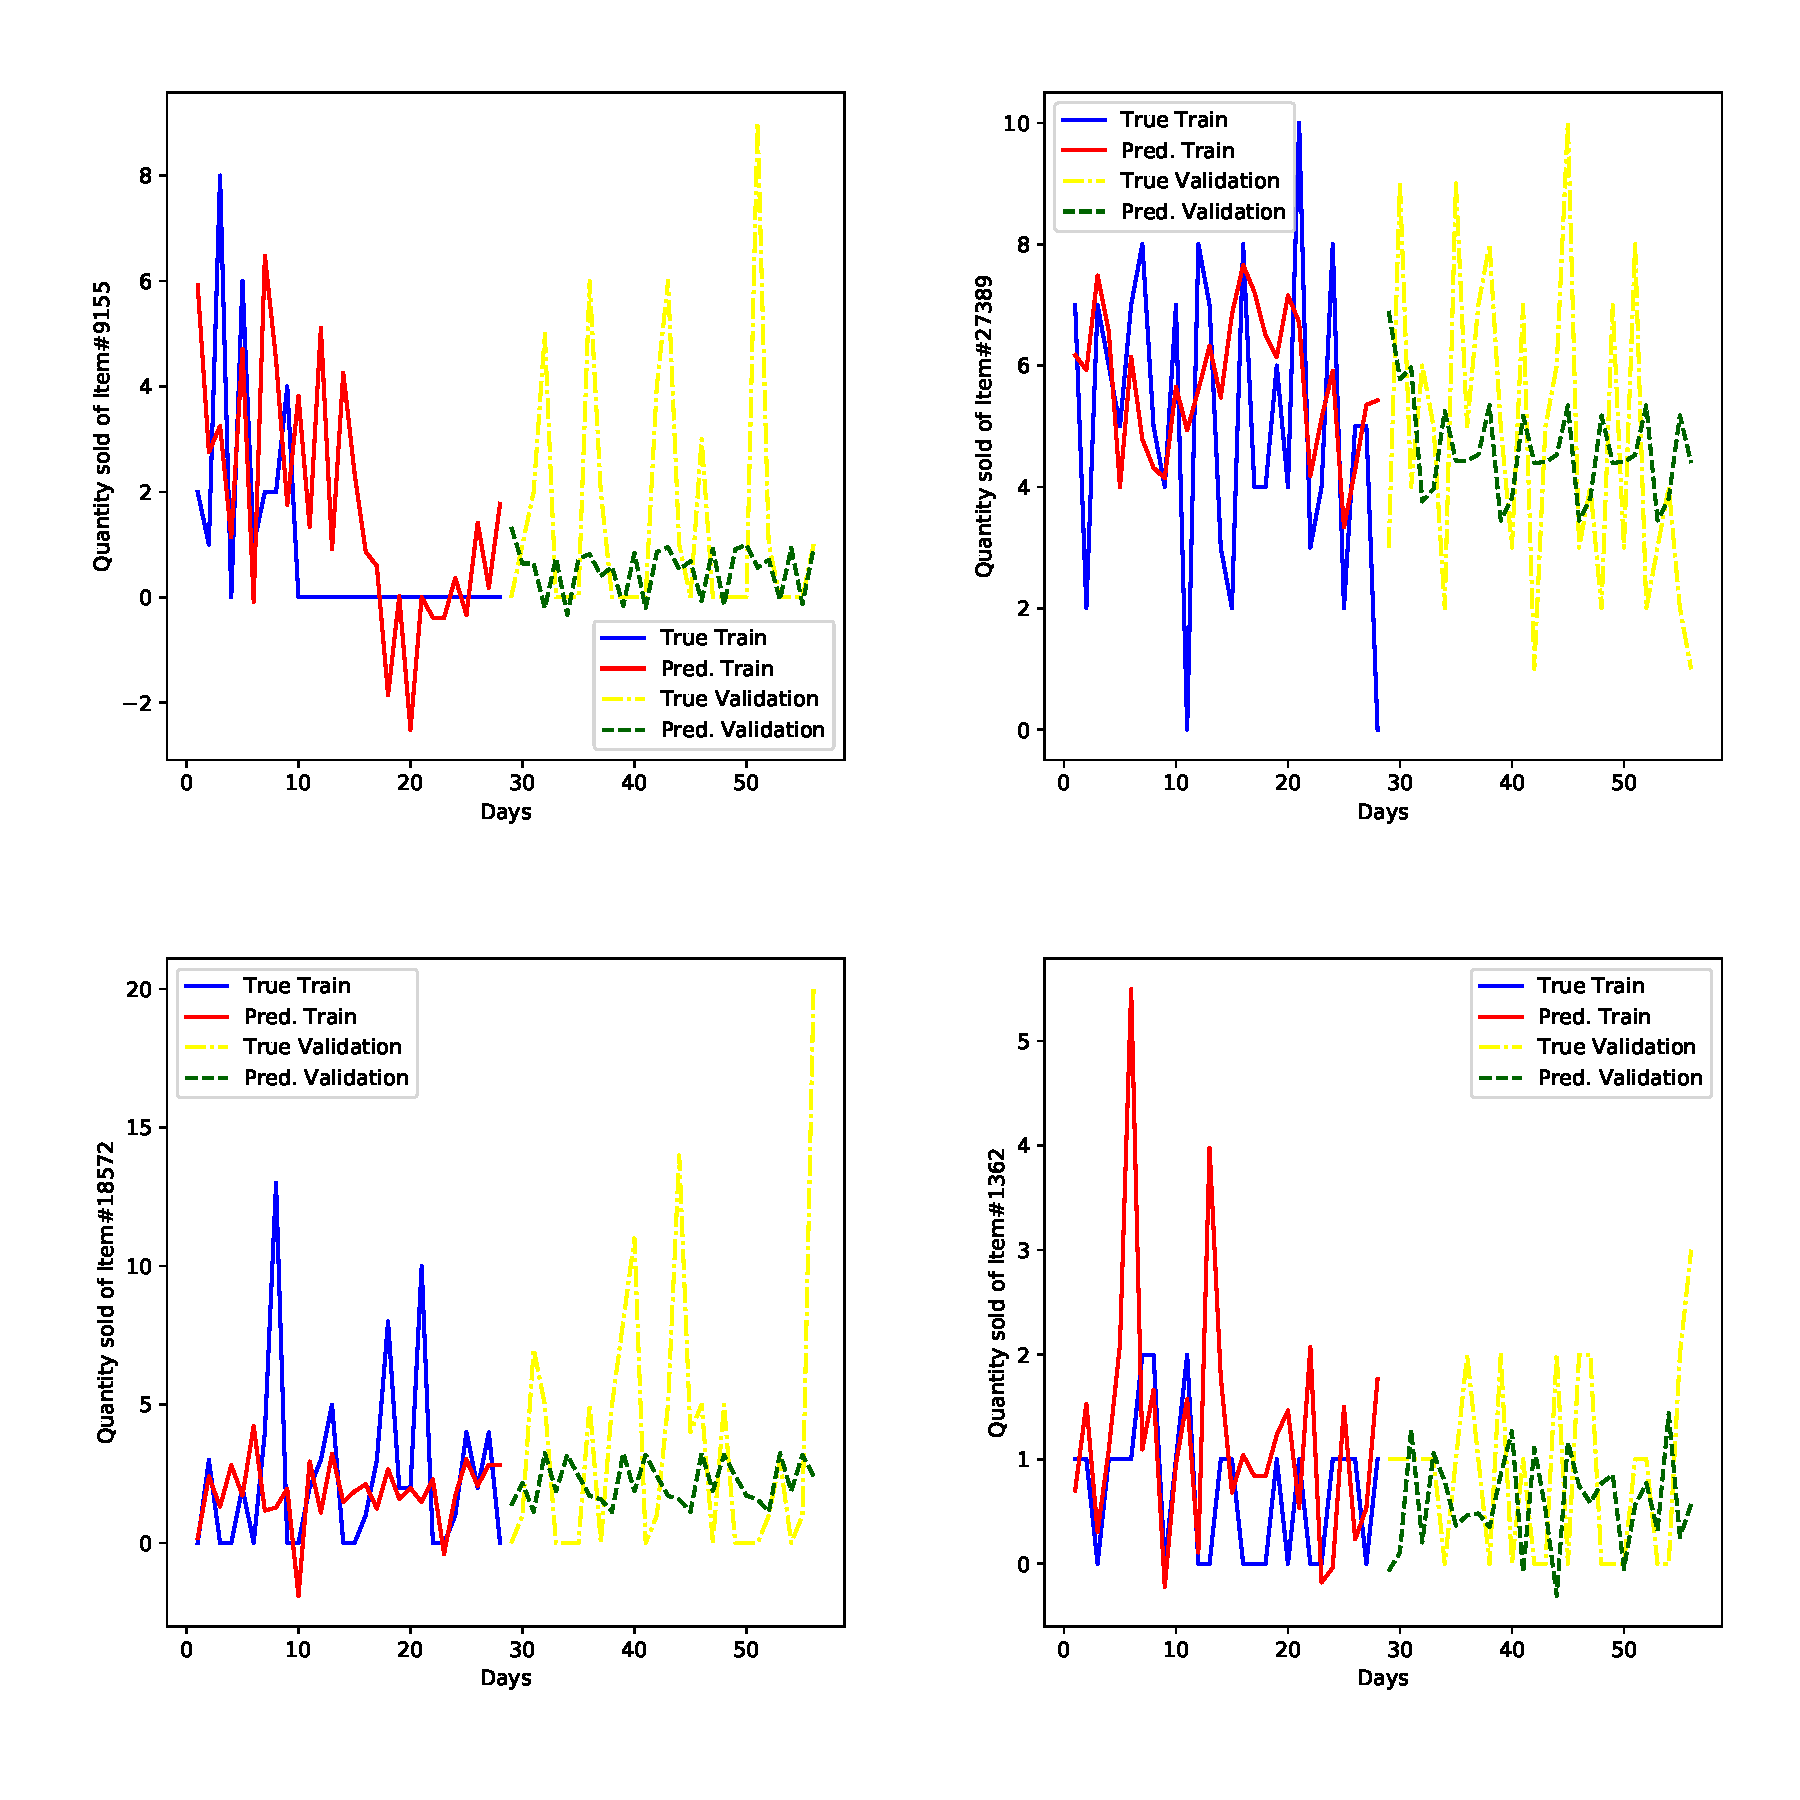
\includegraphics[width=.8\linewidth]{sarimax-items}
  \caption{Item sales as predicted by ARIMA against the ground truth on four randomly chosen items.}
  \label{fig:arima-item-sales}
\end{figure}

\begin{figure}[H]
  \centering
  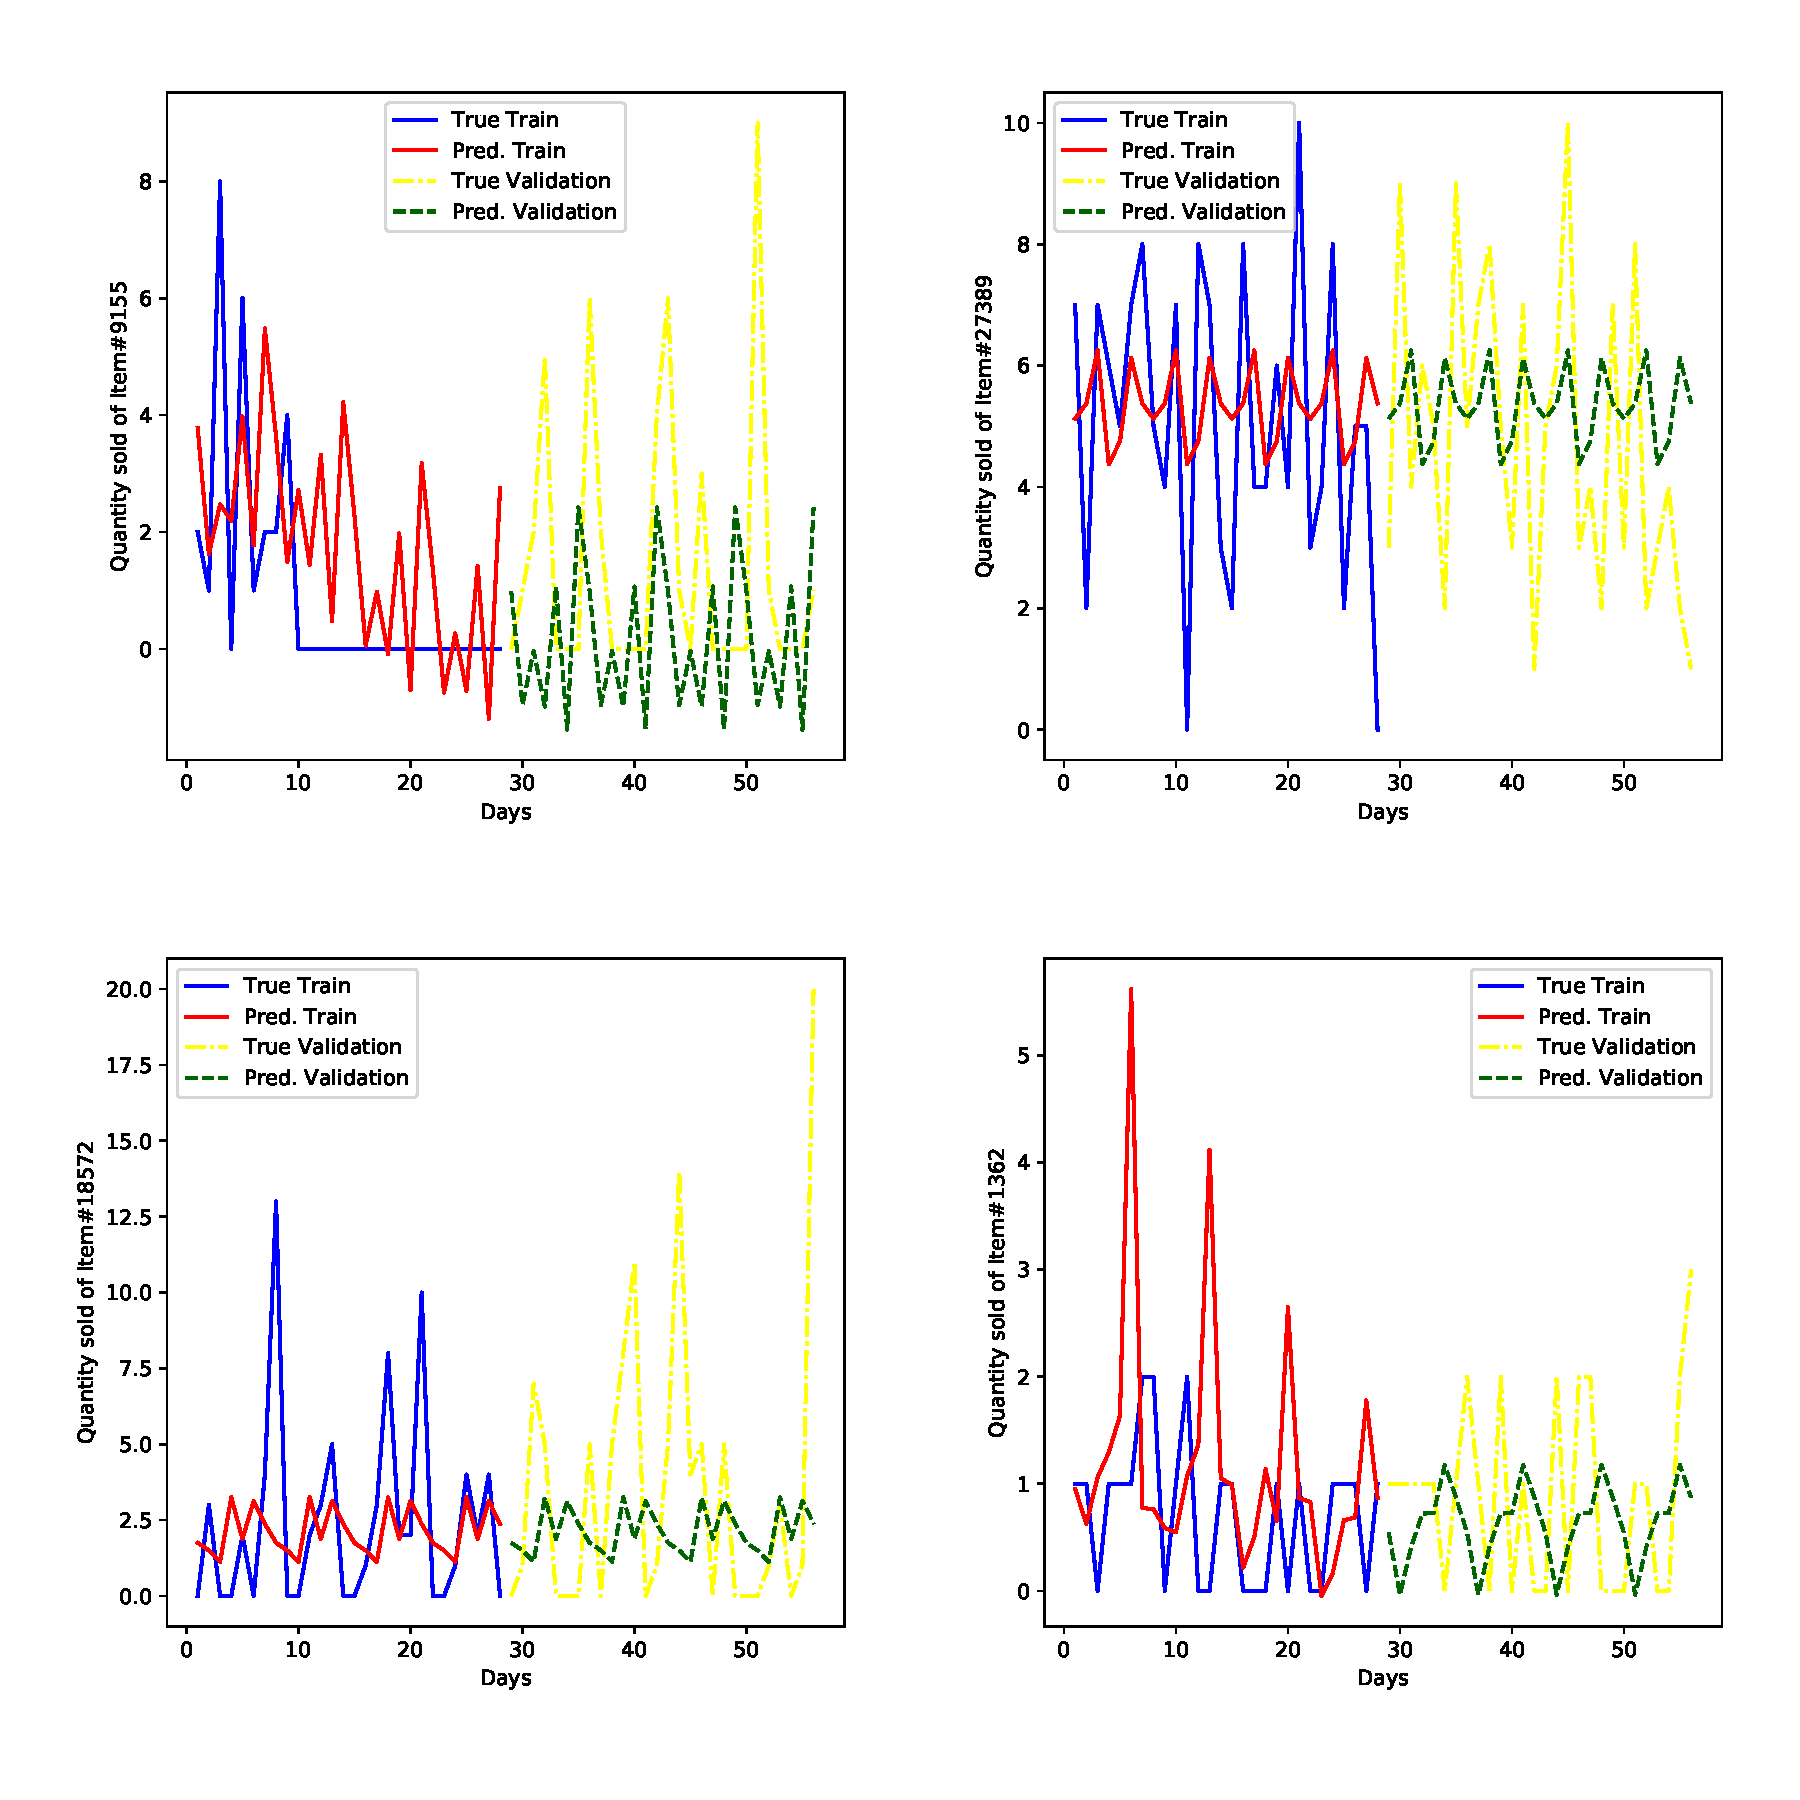
\includegraphics[width=.8\linewidth]{exp-sm-items}
  \caption{Item sales as predicted by ExpSmoothing against the ground truth on four randomly chosen items.}
  \label{fig:expsm-item-sales}
\end{figure}

\begin{figure}[H]
  \centering
  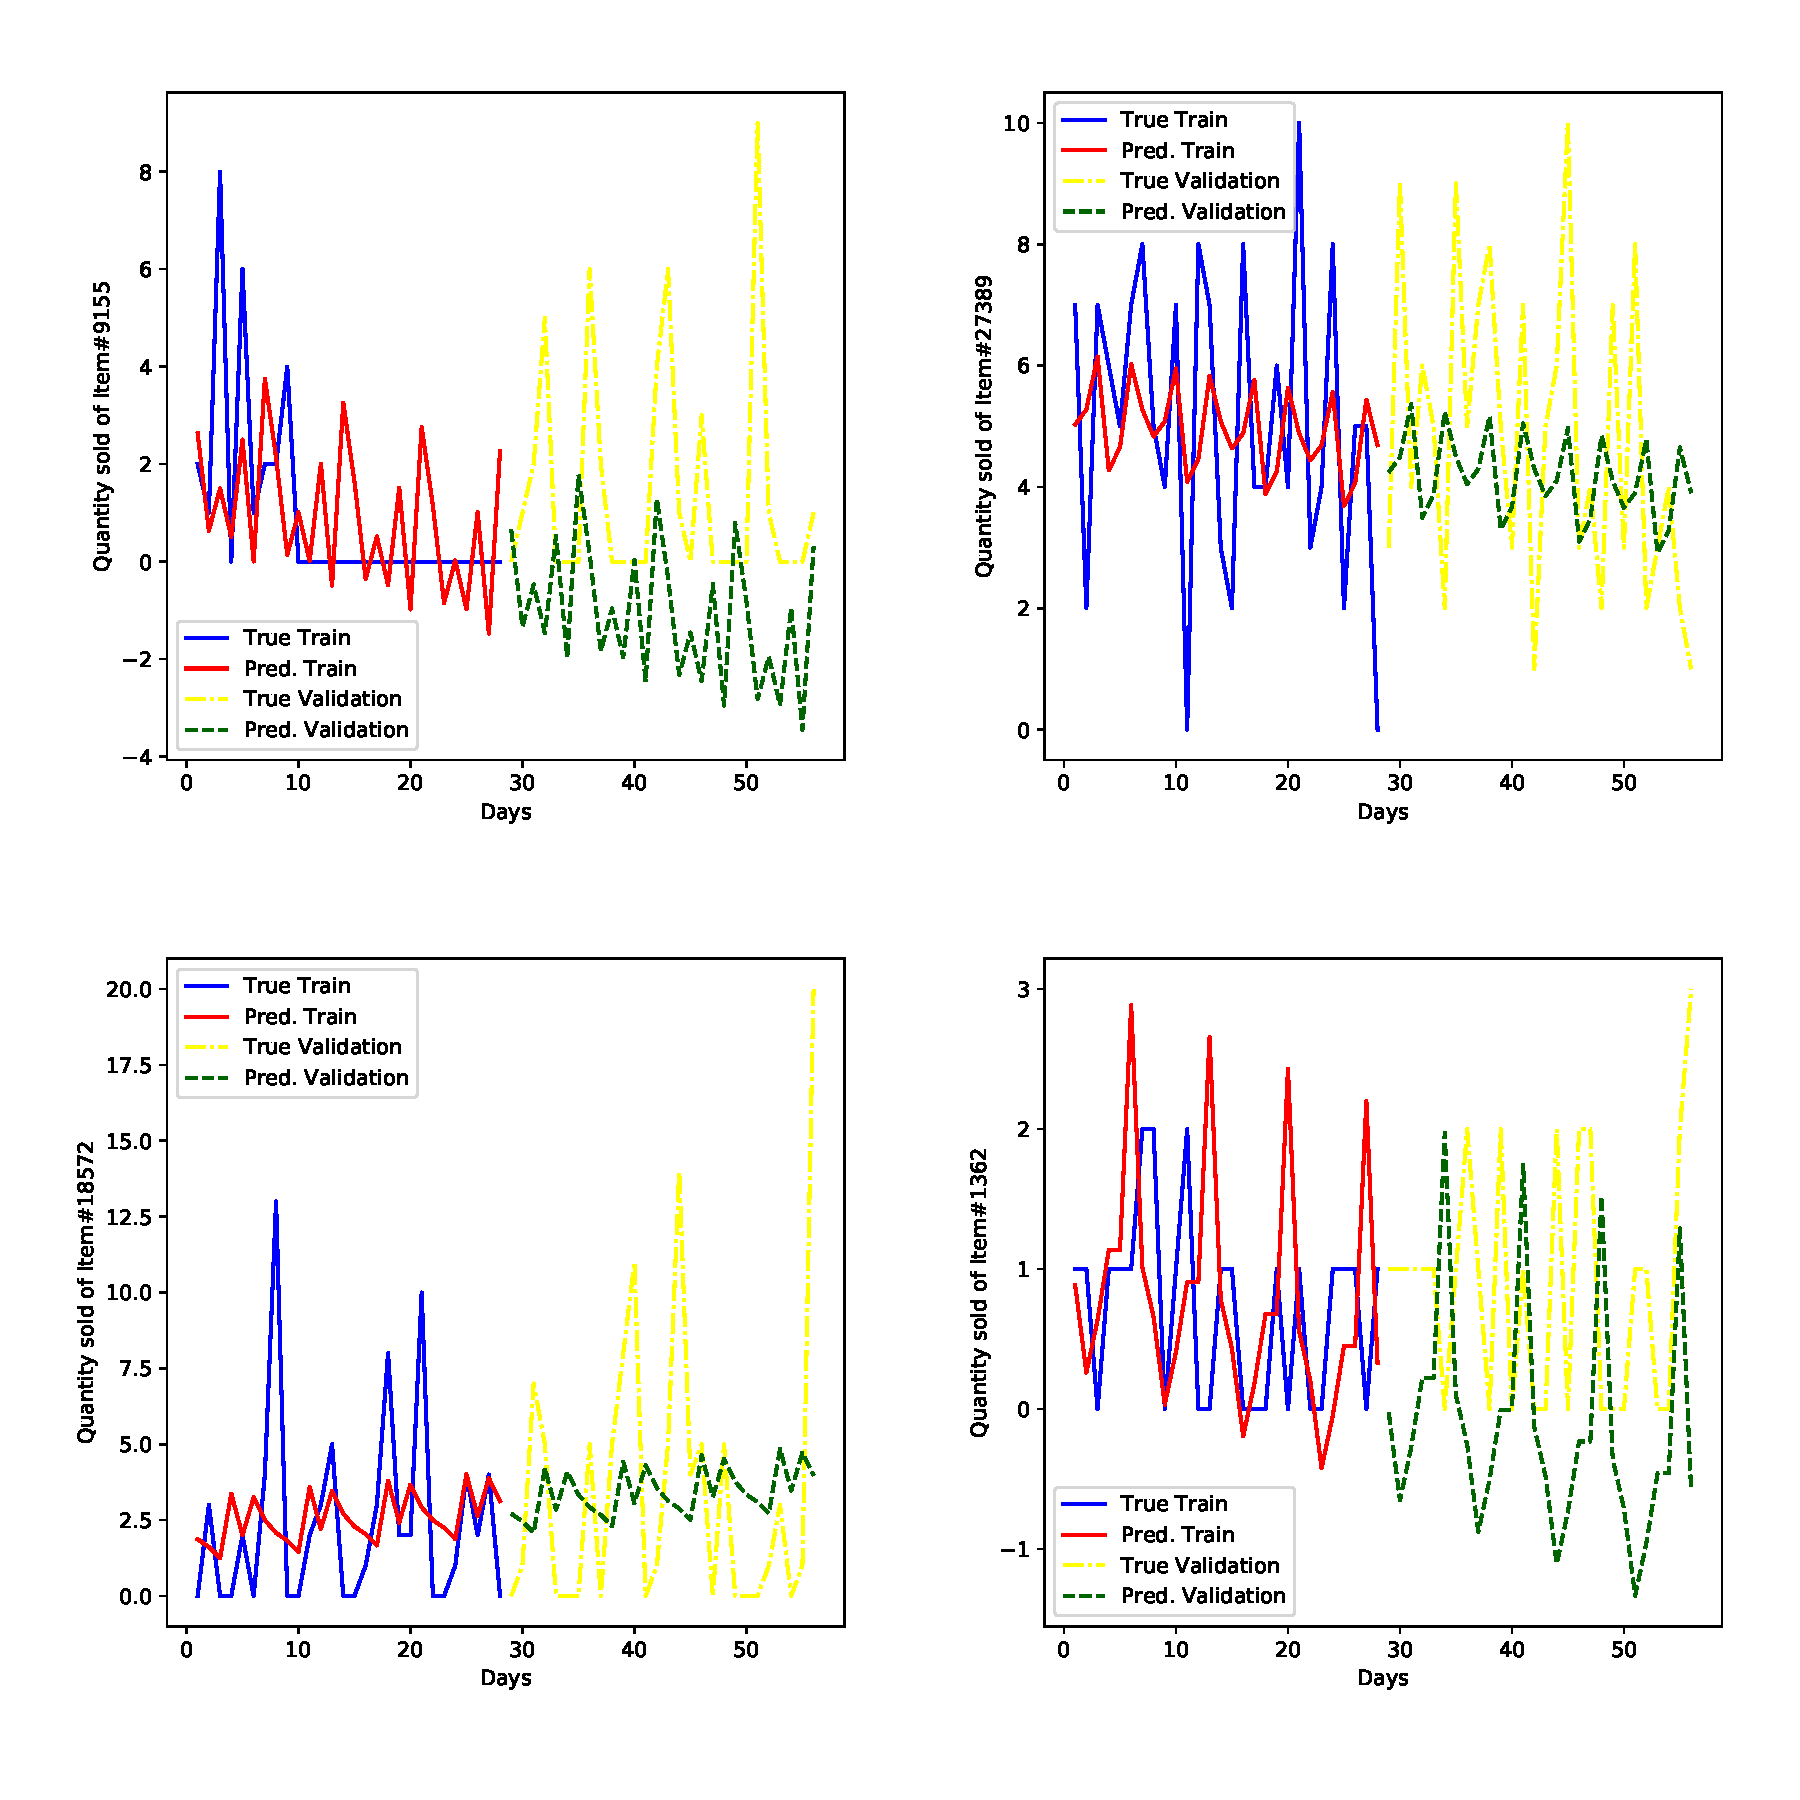
\includegraphics[width=.8\linewidth]{prophet-items}
  \caption{Item sales as predicted by Prophet against the ground truth on four randomly chosen items.}
  \label{fig:pro-item-sales}
\end{figure}

\subsection{Category and State-Level Predictions}
There are three main categories in this dataset: Foods, Hobbies, and Household items, and all items are sold in three states: California, Texas, and Wisconsin. We run forecasting by using the same three models from the previous section but this time we try to predict the volume of sells in each item category as well as in each state. As the number of item categories ($3$) and the number of states ($3$) is manageable, we were able to train using the entire history of observations for this task. The root mean squared errors are tabulated in \Cref{tab:rmse-category,tab:rmse-state}. Surprisingly, we see that Prophet performs best on this task, and this is because the quantity of data is too large for a single smoothing parameter to capture well (as in ExpSmoothing) and because Prophet models seasonality by a stronger model than ARIMA. Compared to the items (where we used only $28 \times 4$ days), here we use the entire history (about $1900$ days). We plot the time series predictions for the last 28 days of the training set and forecast 28 days into the future in \Cref{fig:arima-category-sales,fig:expsm-category-sales,fig:pro-category-sales} for categories and \Cref{fig:arima-state-sales,fig:expsm-state-sales,fig:pro-state-sales} for states. We observe that the closest fit is Prophet, followed by ARIMA and ExpSmooth.

\begin{table}[]
  \centering
  \caption{Root Mean Square Error for category-level prediction by method.}
  \label{tab:rmse-category}
  \begin{tabular}{cc}
  \hline
  Model Used   & Root Mean Square Error \\ \hline
  ARIMA        & $6.8457$               \\
  ExpSmoothing & $7.0749$               \\
  Prophet      & $6.4010$               \\ \hline
  \end{tabular}
\end{table}

\begin{table}[]
    \centering
    \caption{Root Mean Square Error for state-level prediction by method.}
    \label{tab:rmse-state}
    \begin{tabular}{cc}
    \hline
    Model Used   & Root Mean Square Error \\ \hline
    ARIMA        & $5.5871$               \\
    ExpSmoothing & $5.9941$               \\
    Prophet      & $5.4918$               \\ \hline
    \end{tabular}
  \end{table}


\begin{figure}[H]
  \centering
  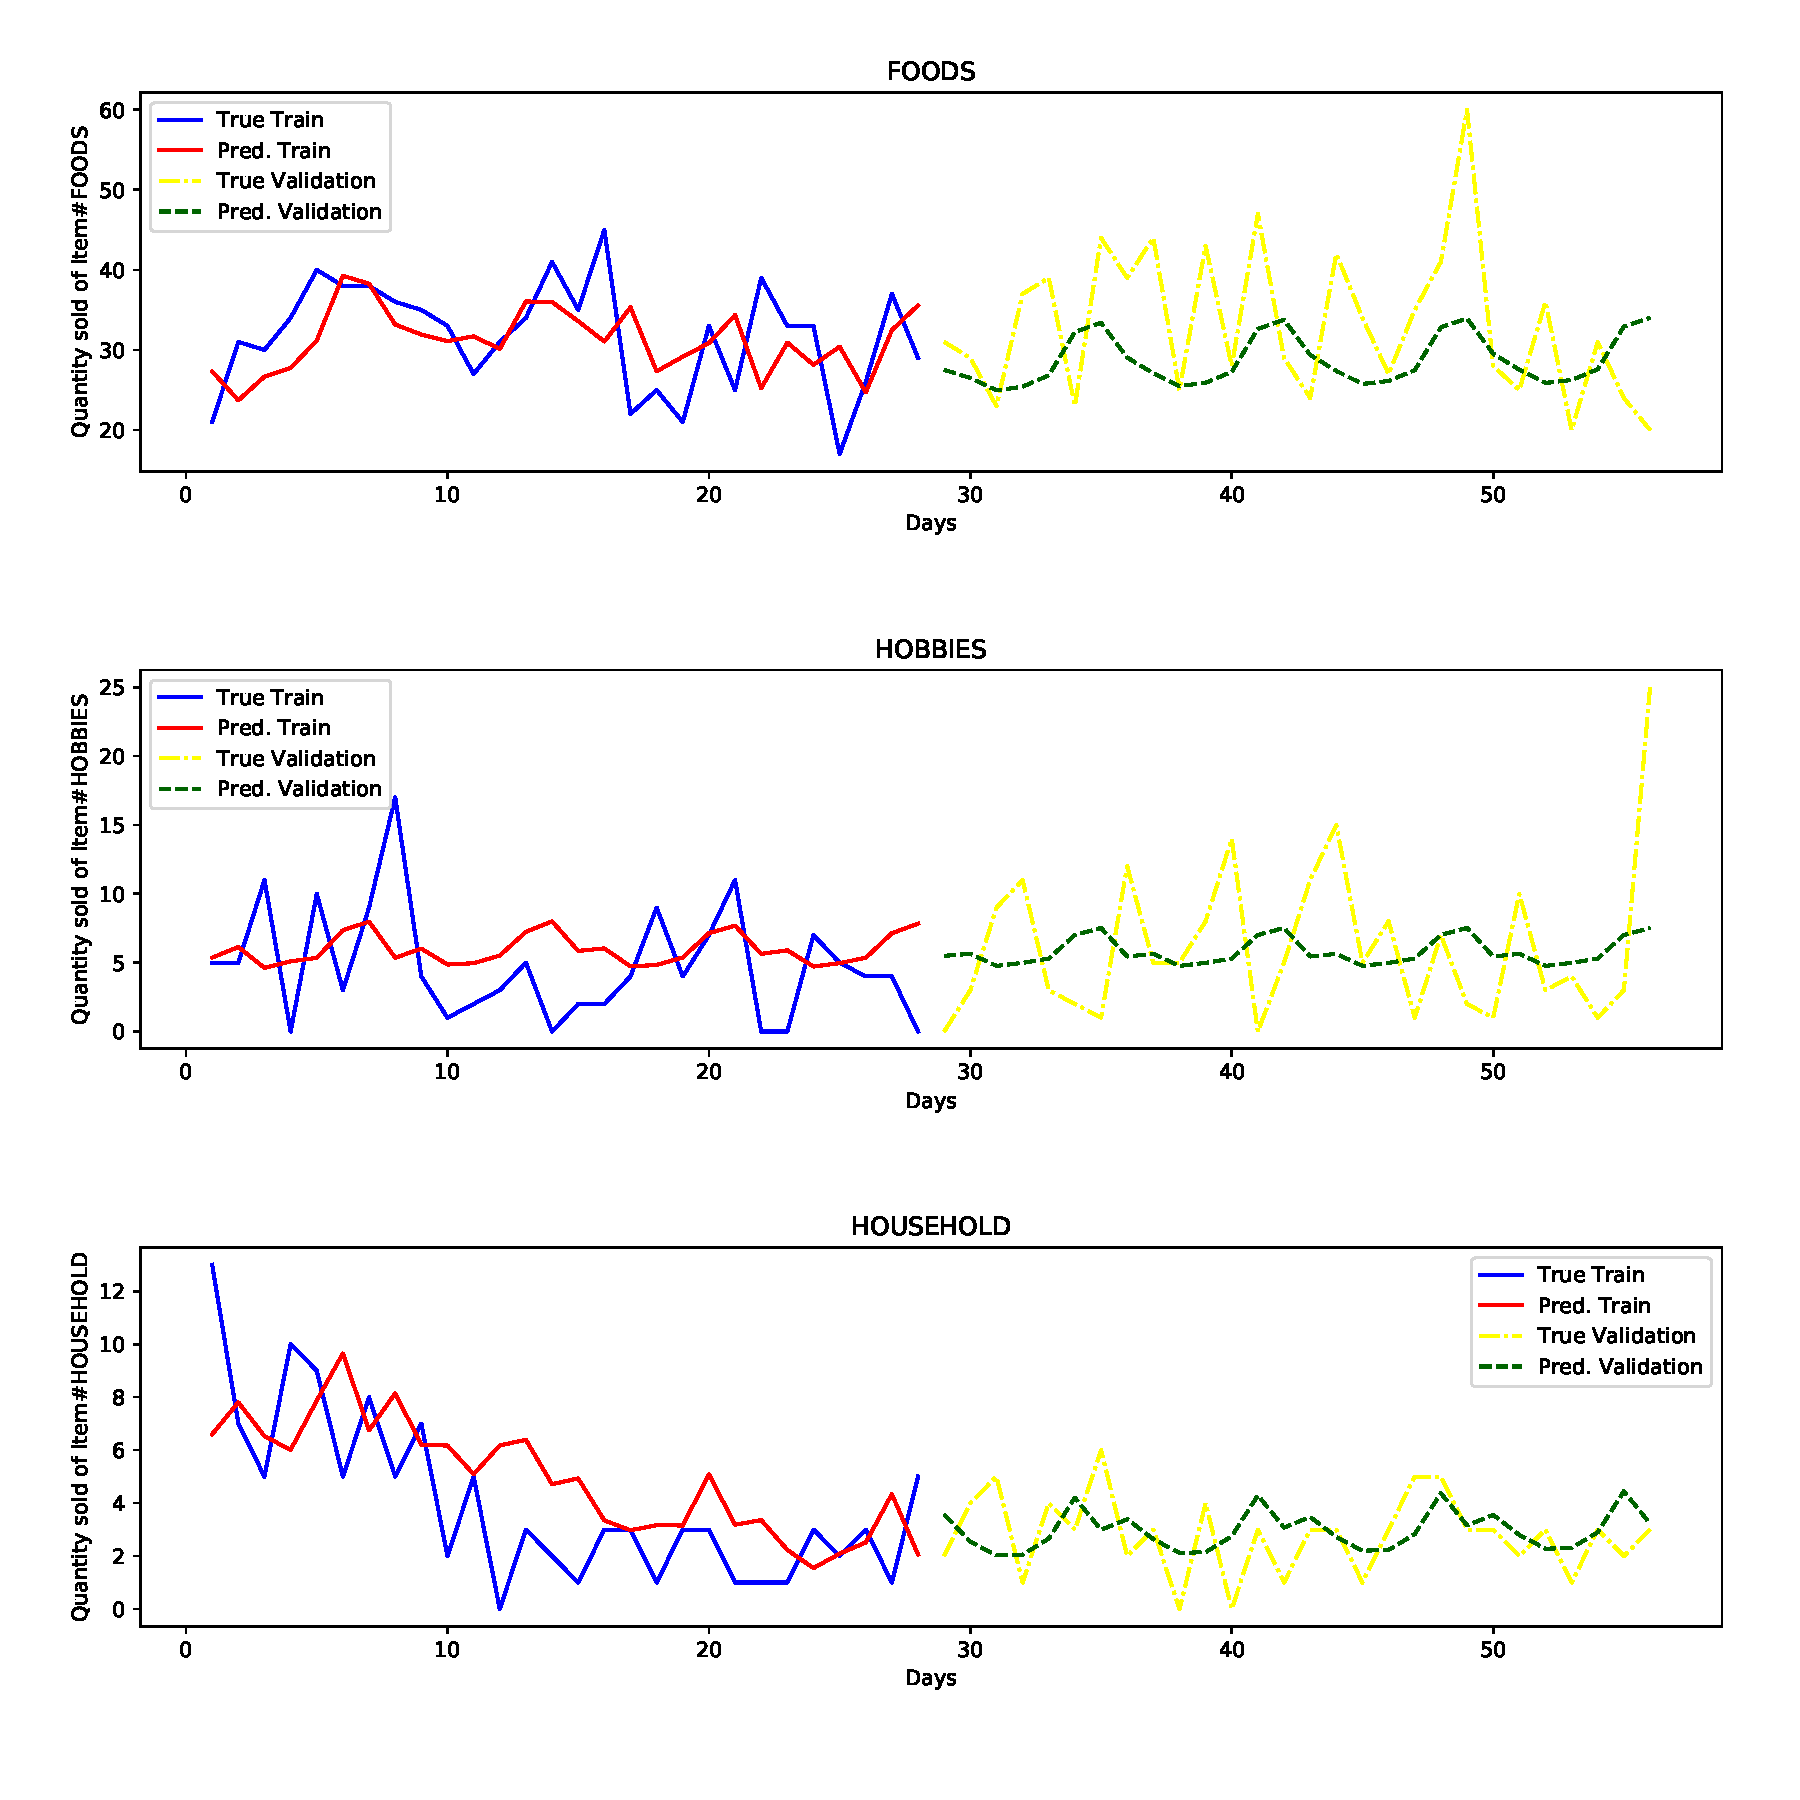
\includegraphics[width=.8\linewidth]{sarimax-cat}
  \caption{Item sales per category as predicted by ARIMA against the ground truth.}
  \label{fig:arima-category-sales}
\end{figure}

\begin{figure}[H]
  \centering
  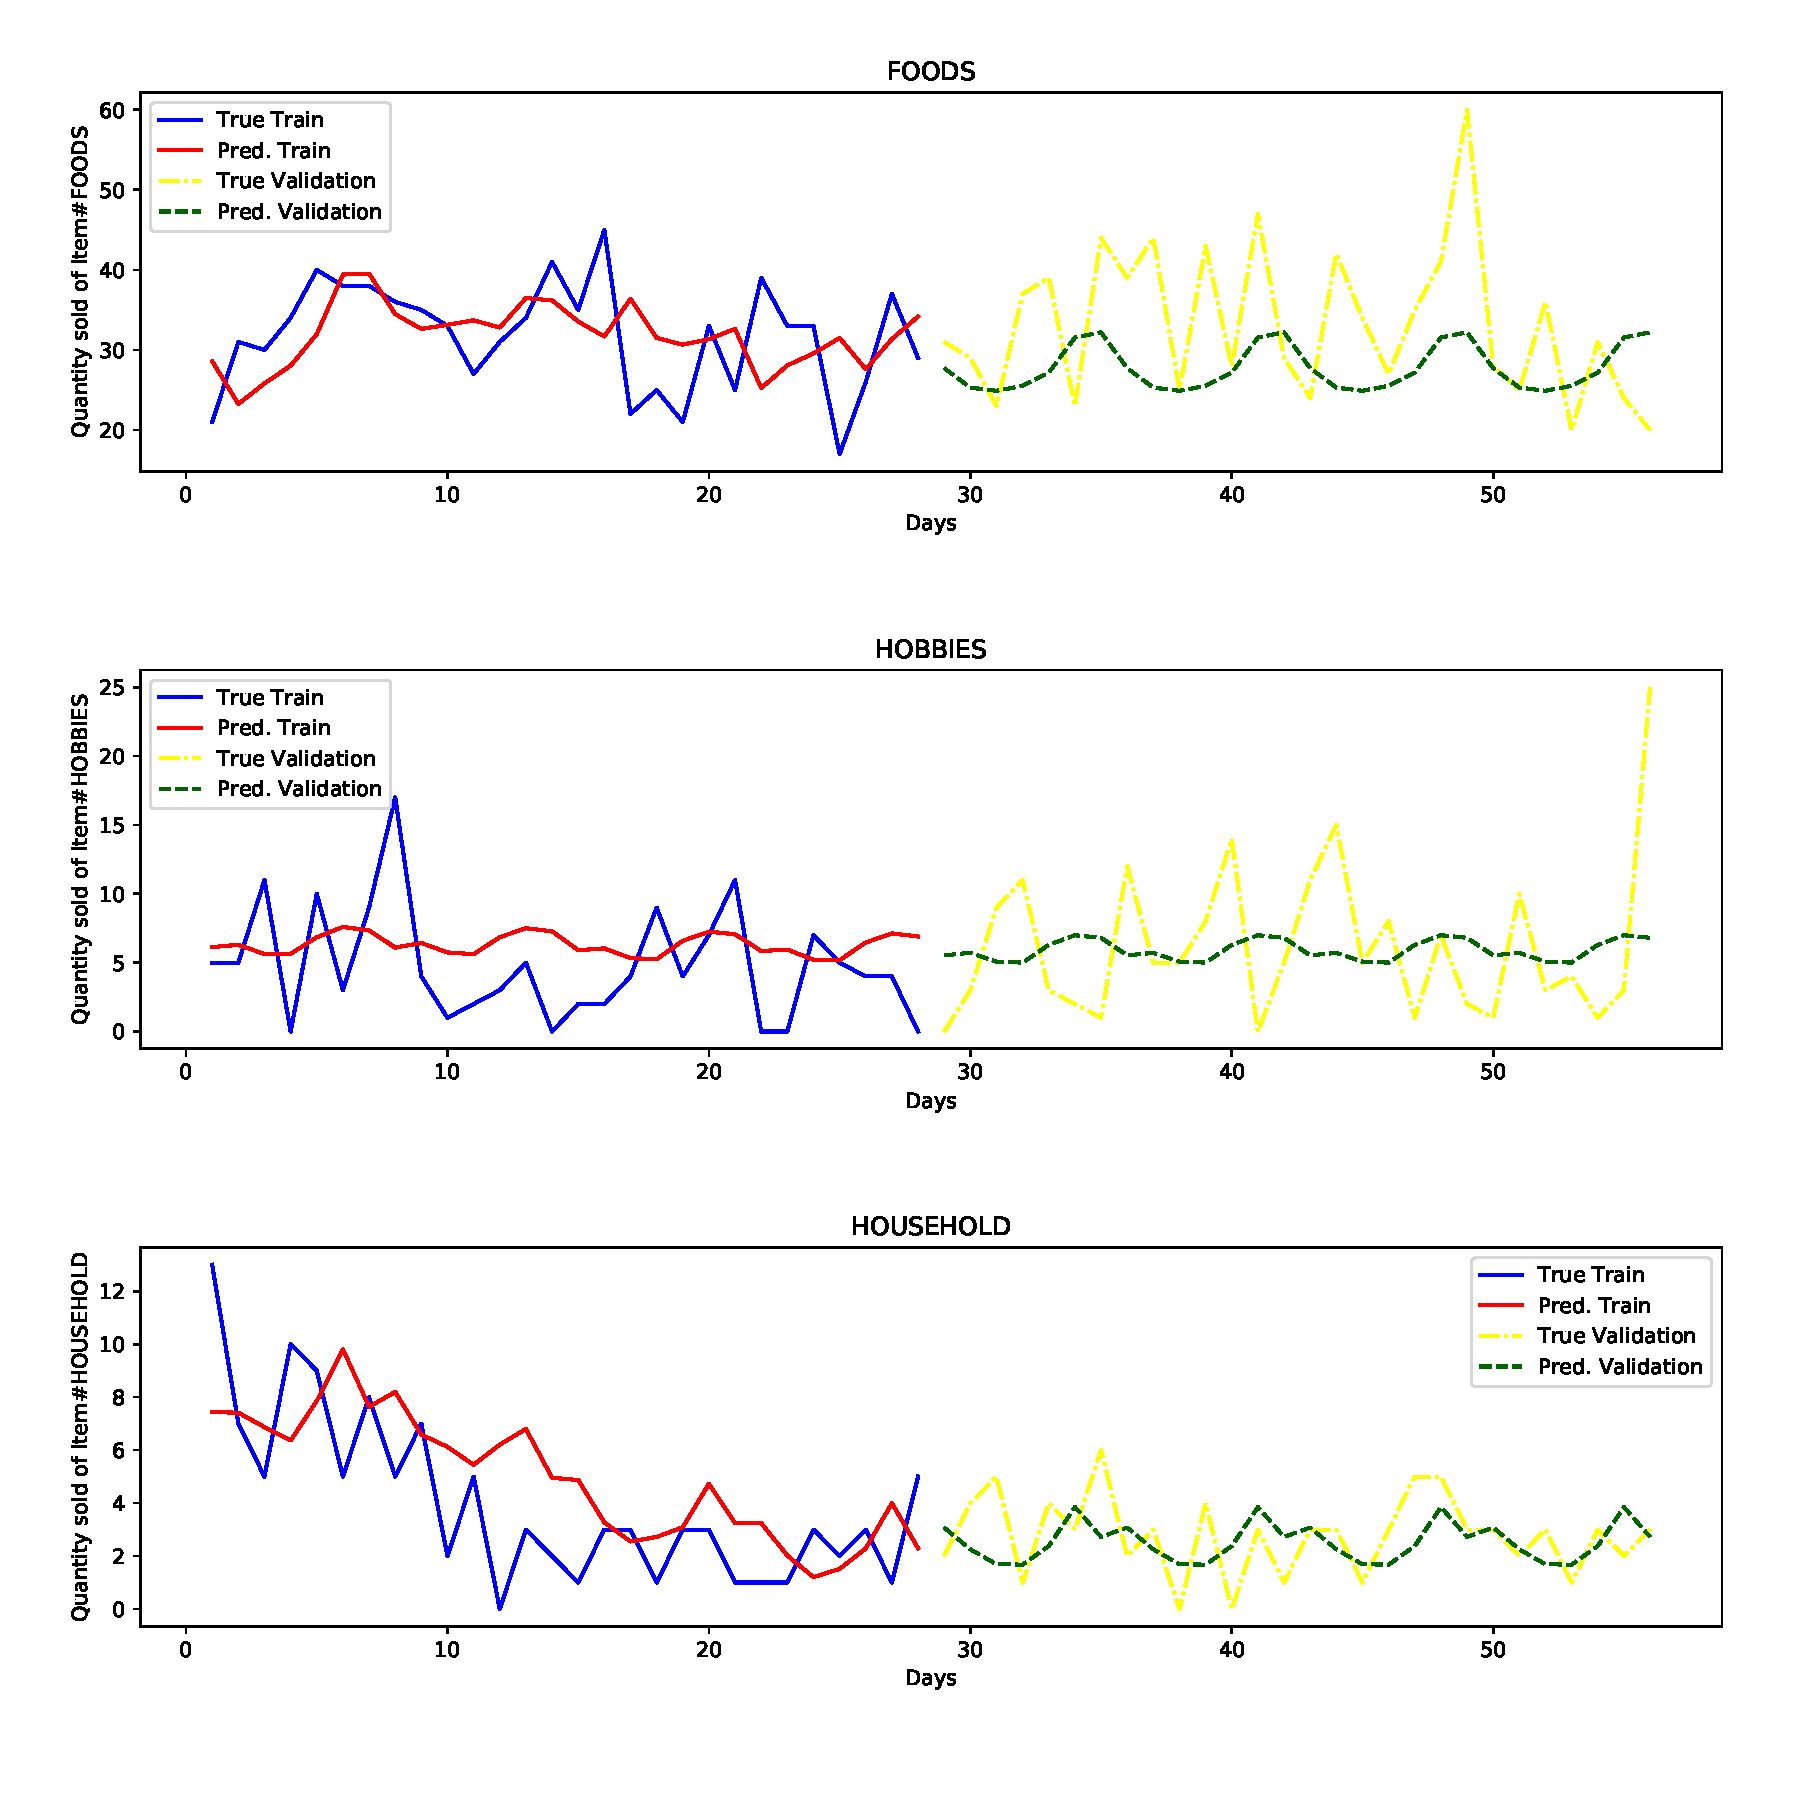
\includegraphics[width=.8\linewidth]{exp-sm-cat}
  \caption{Item sales per category as predicted by ExpSmoothing against the ground truth.}
  \label{fig:expsm-category-sales}
\end{figure}

\begin{figure}[H]
  \centering
  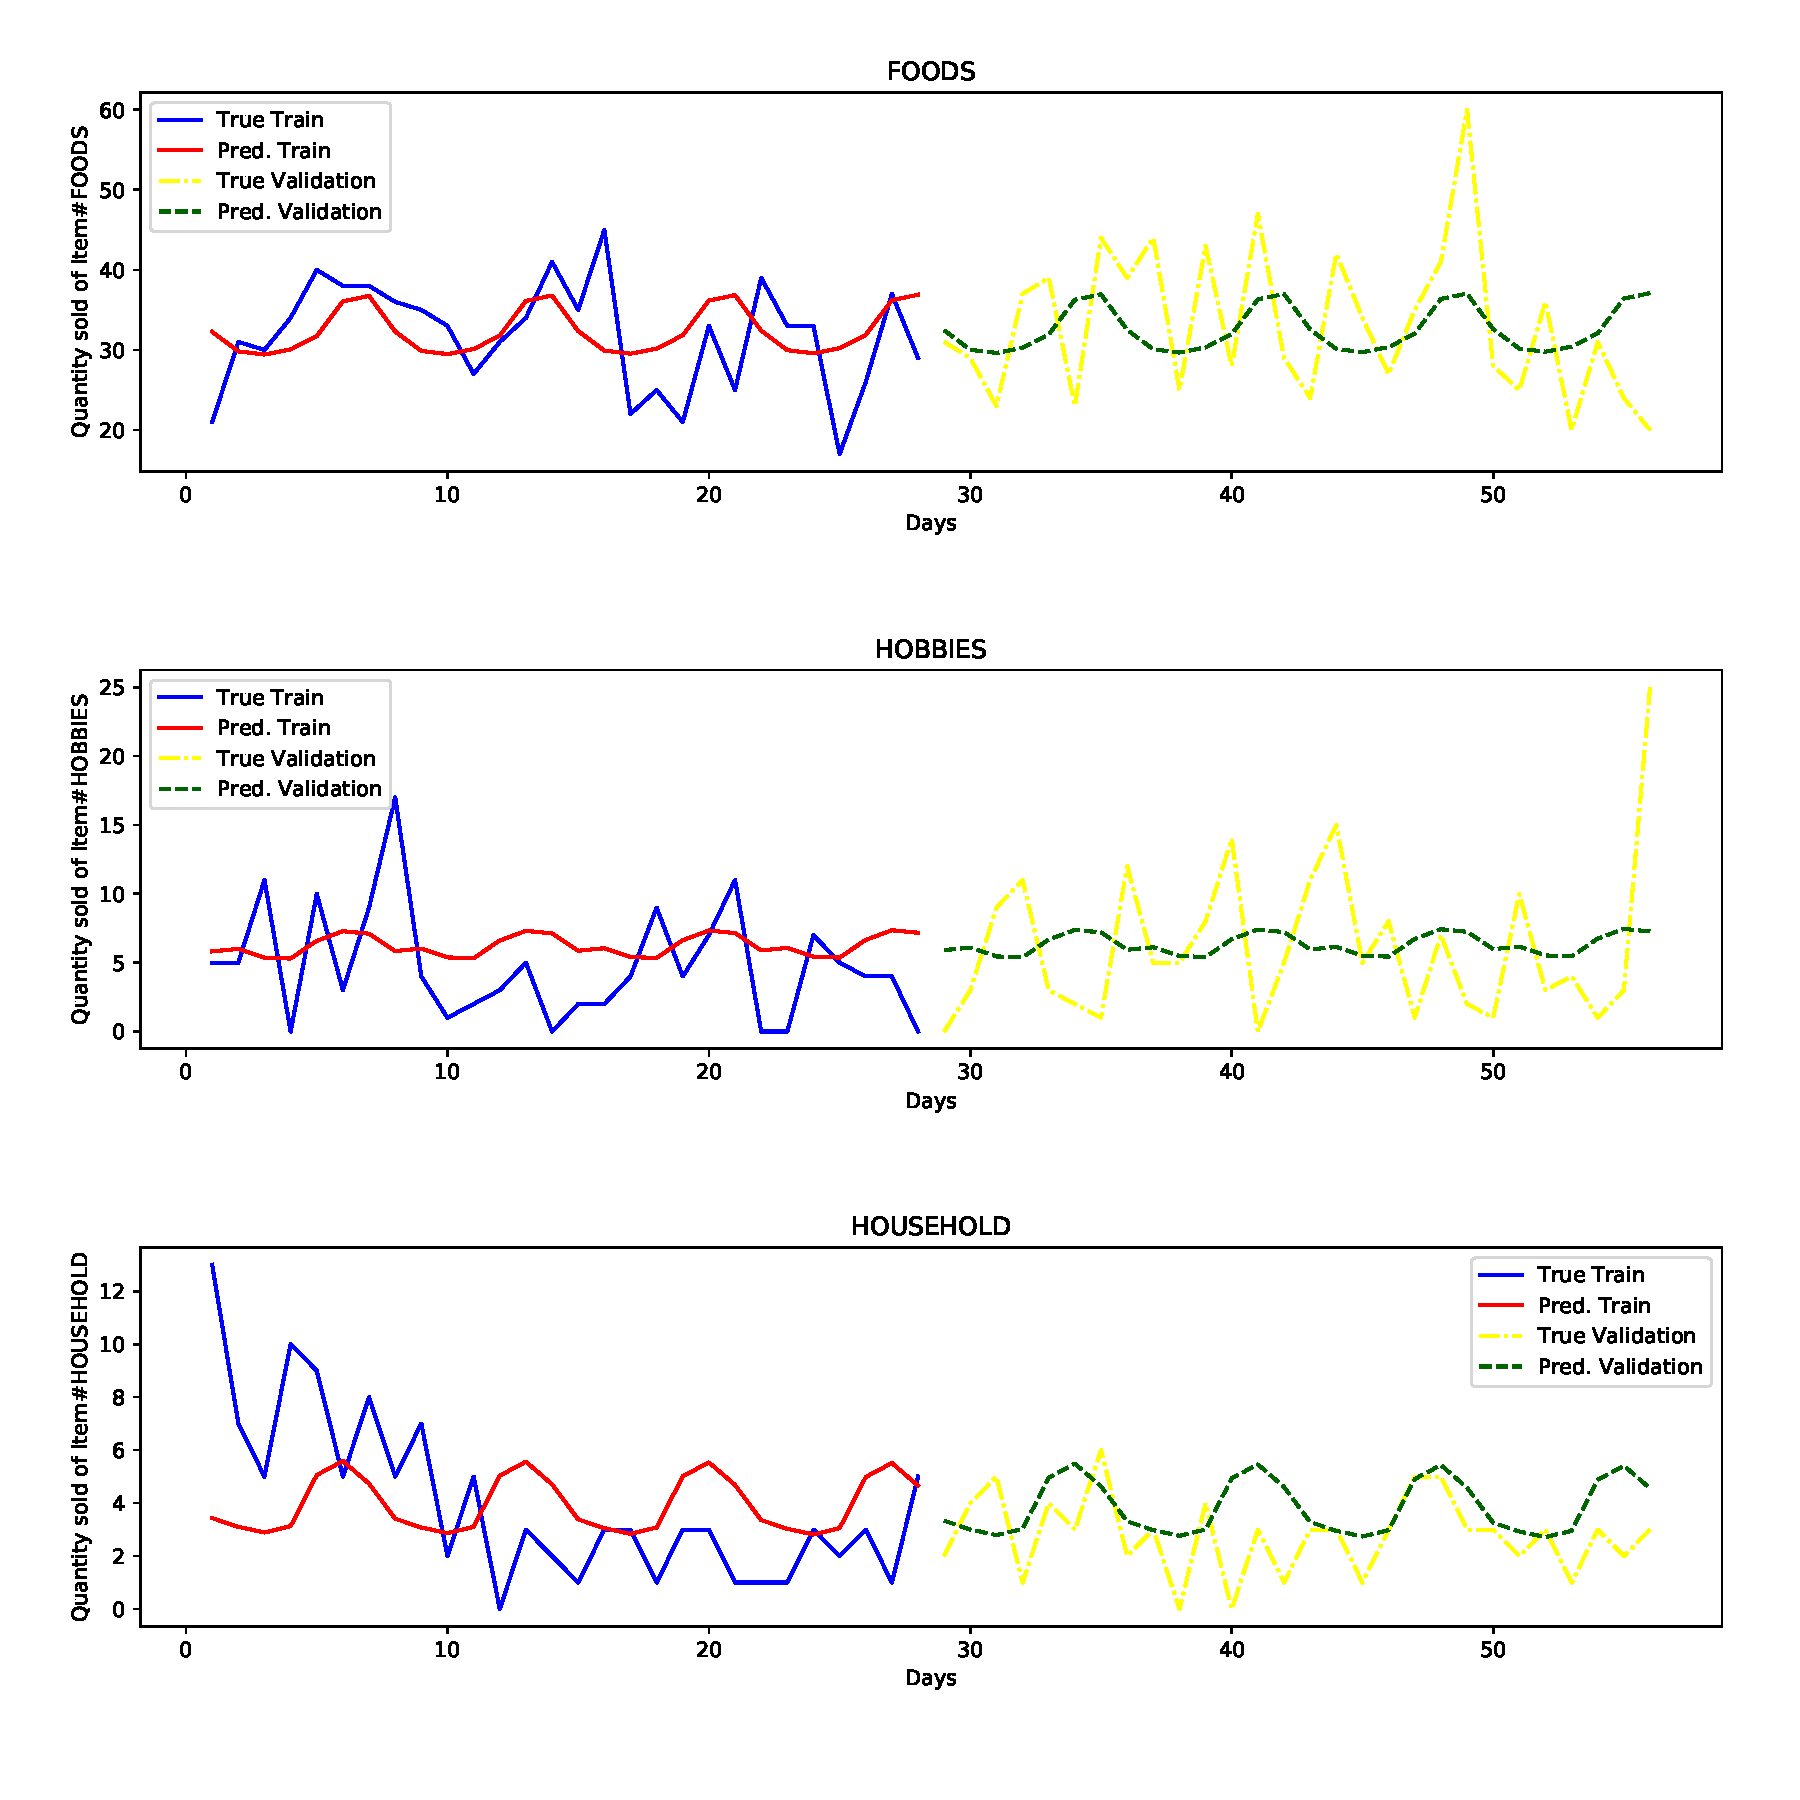
\includegraphics[width=.8\linewidth]{pro-cat}
  \caption{Item sales per category as predicted by Prophet against the ground truth.}
  \label{fig:pro-category-sales}
\end{figure}

\begin{figure}[H]
  \centering
  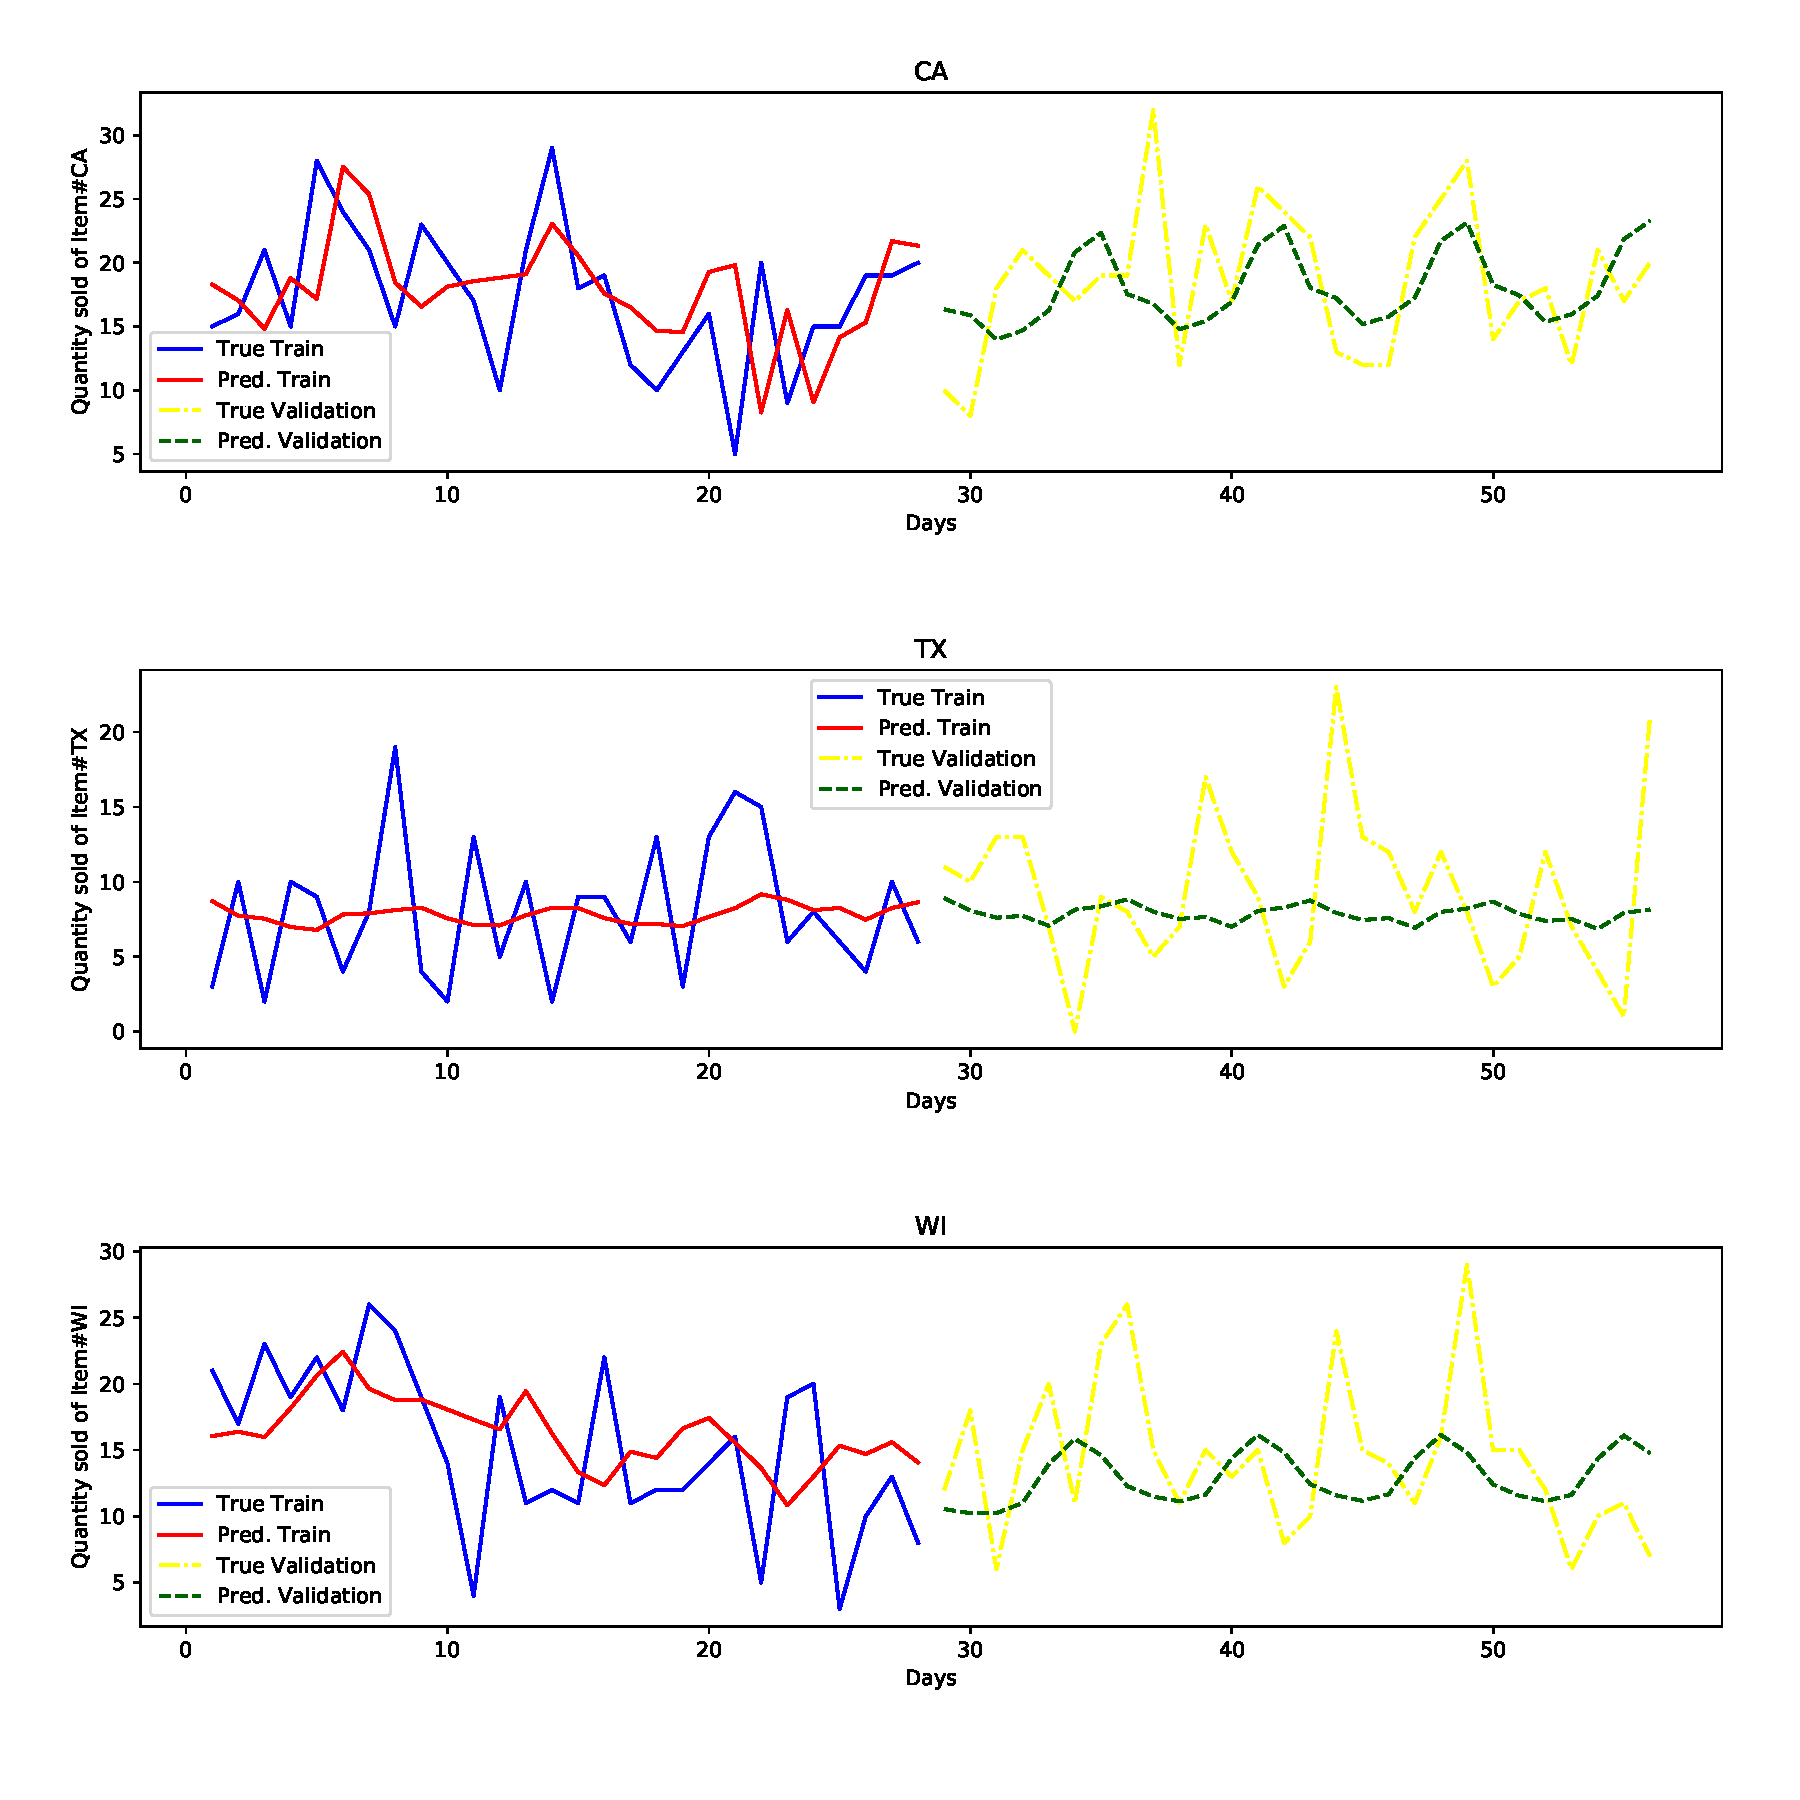
\includegraphics[width=.8\linewidth]{sarimax-state}
  \caption{Item sales per state as predicted by ARIMA against the ground truth.}
  \label{fig:arima-state-sales}
\end{figure}

\begin{figure}[H]
  \centering
  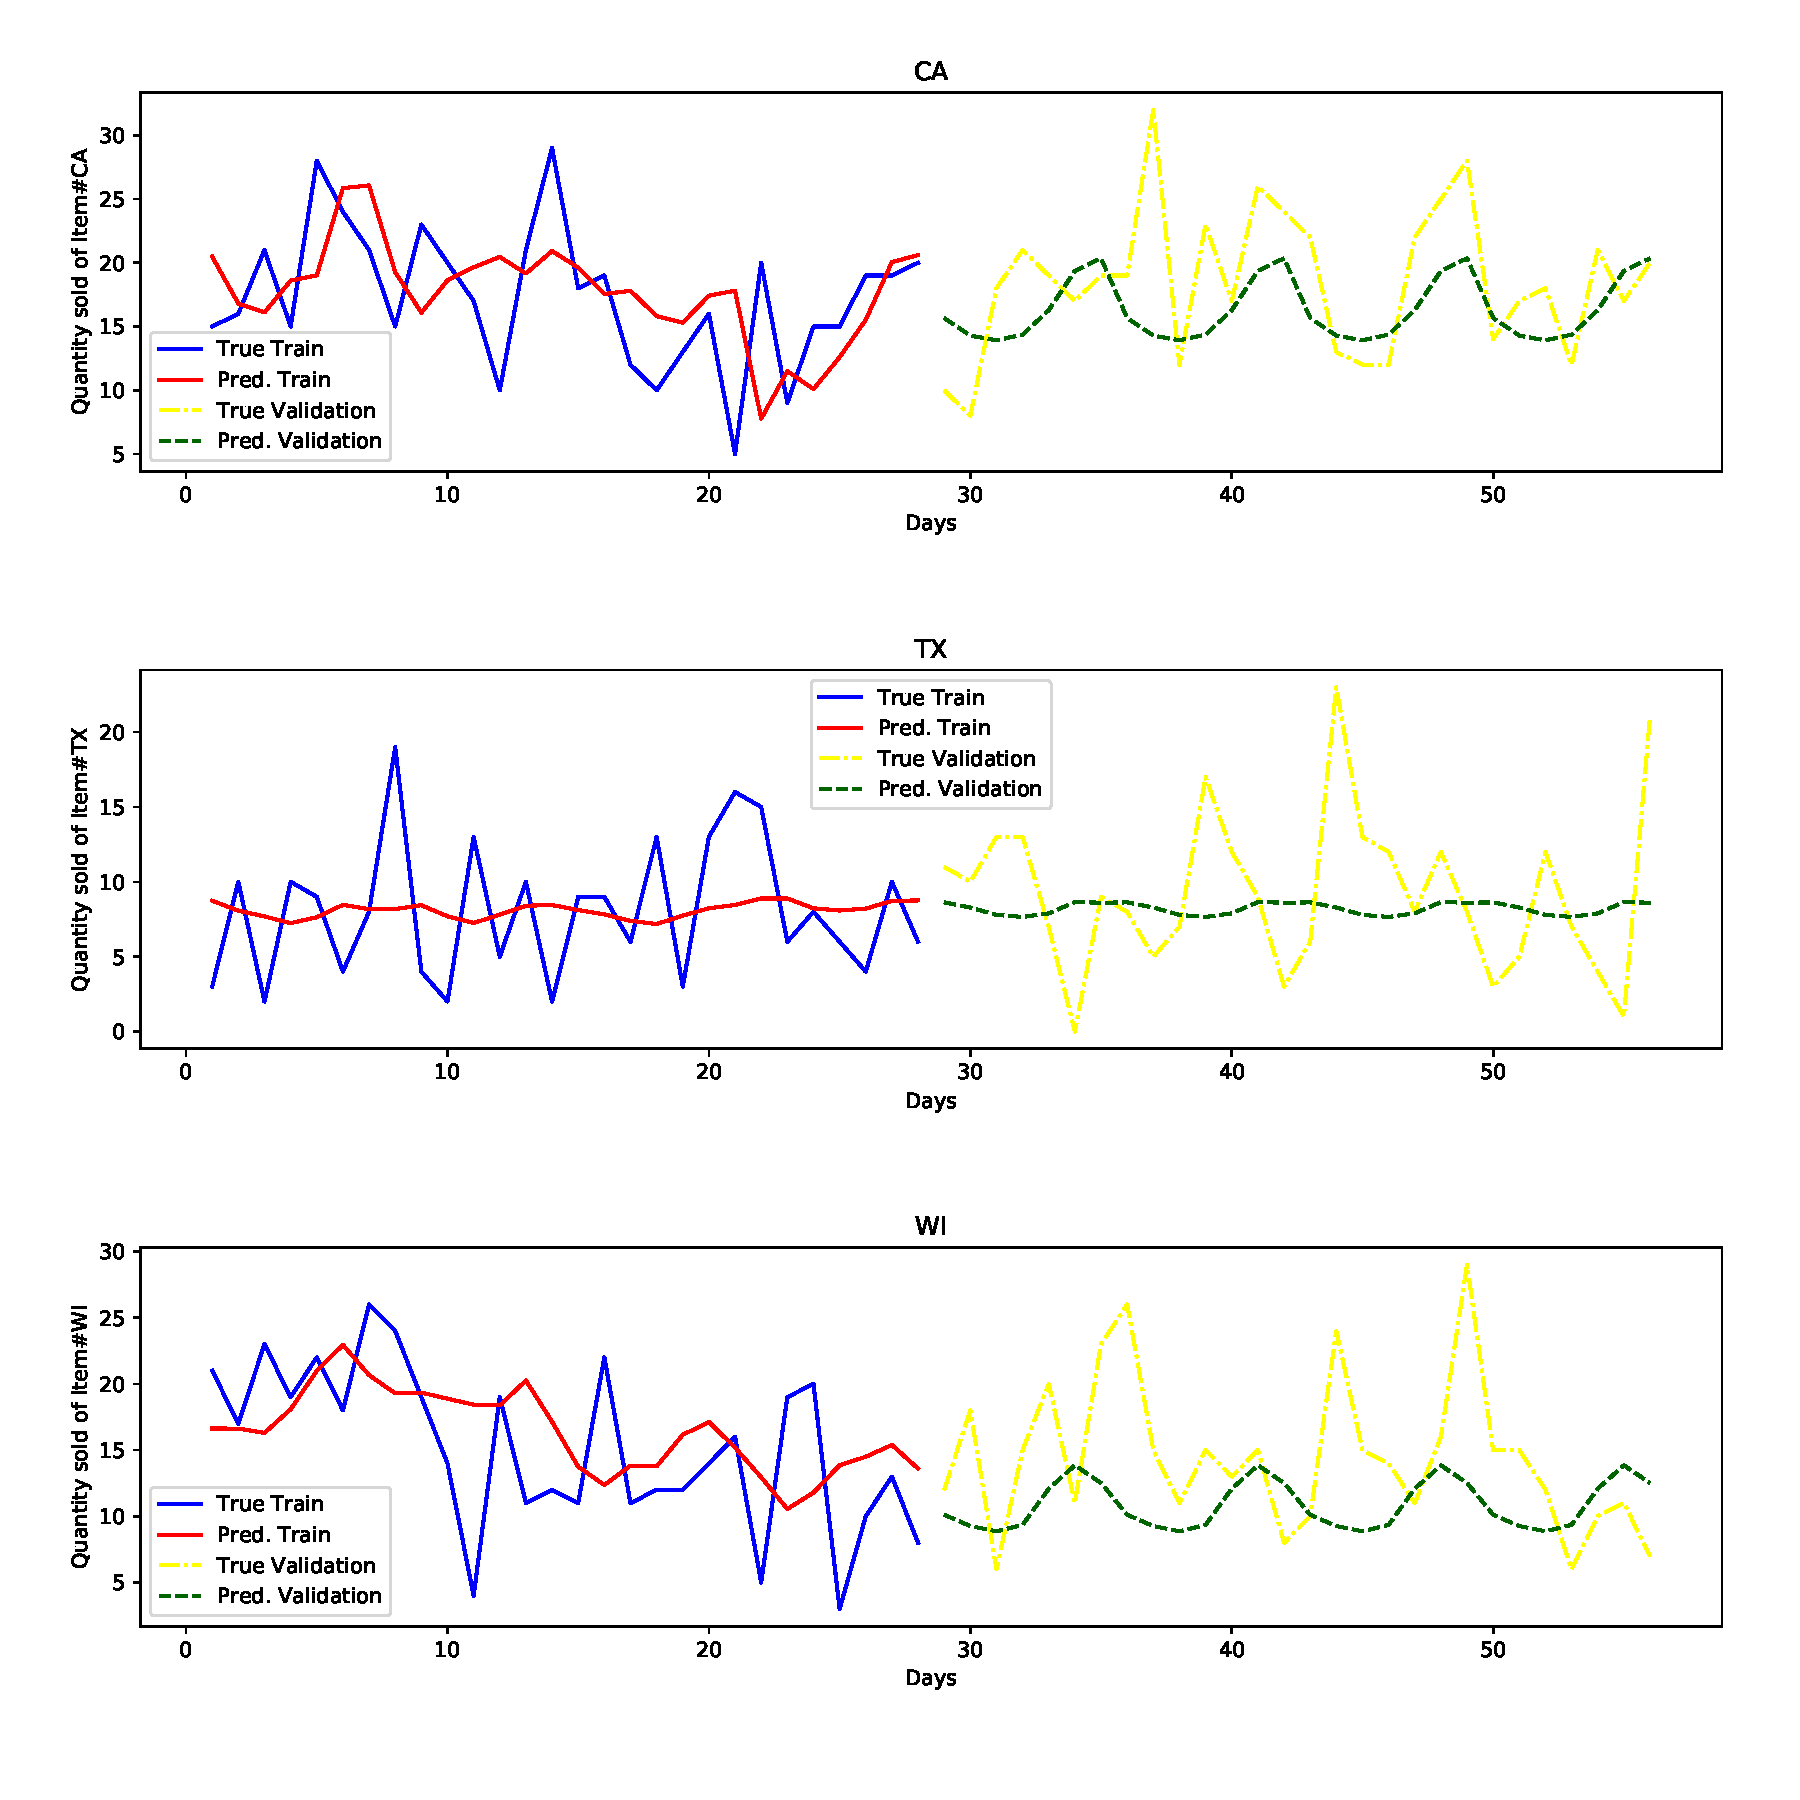
\includegraphics[width=.8\linewidth]{exp-sm-state}
  \caption{Item sales per state as predicted by ExpSmoothing against the ground truth.}
  \label{fig:expsm-state-sales}
\end{figure}

\begin{figure}[H]
  \centering
  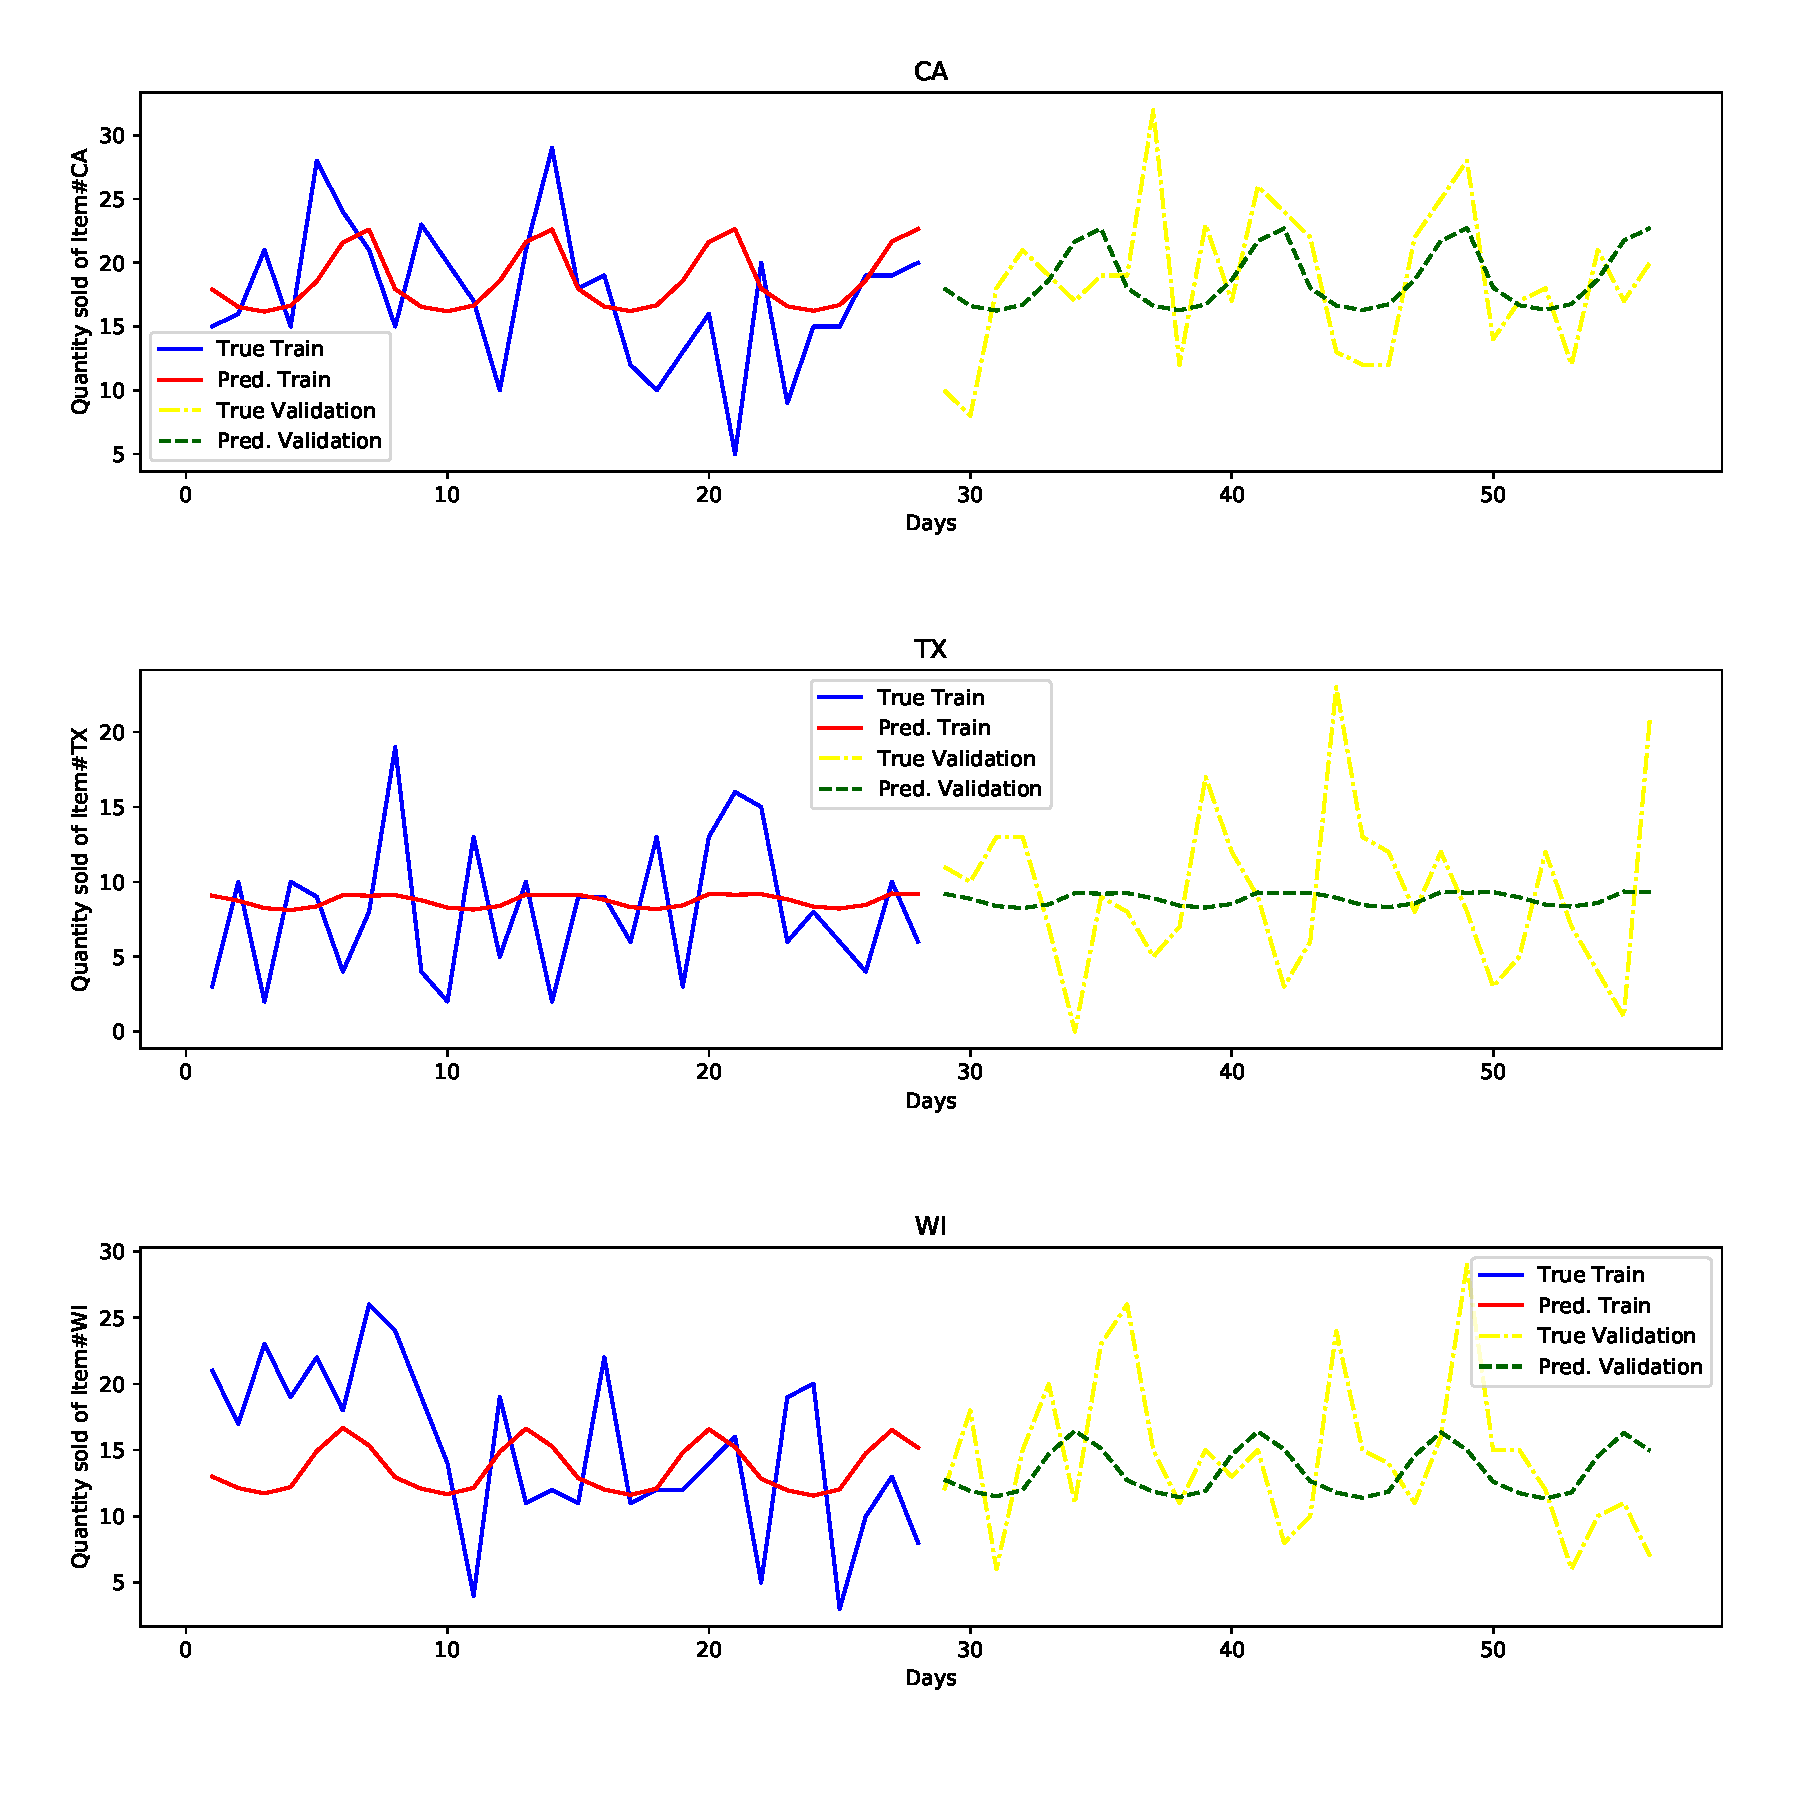
\includegraphics[width=.8\linewidth]{pro-state}
  \caption{Item sales per state as predicted by Prophet against the ground truth.}
  \label{fig:pro-state-sales}
\end{figure}

\subsection{Other approaches and future Work}
We tried to implement prediction using recurrent neural networks, but it was too difficult and we could not get it working on time. We also did not use any ensembles, when eighty percent of the winning models from last year's competition (the M4 competition) were ensembles. In future work on time series forecasting (in this competition or otherwise), we will consider using ensembles.

\bibliography{main}

\end{document}